%
% Cura.tex
%
% LulzBot Cura User Manual
%
% Copyright (C) 2016 Aleph Objects, Inc.
%
% This document is licensed under the Creative Commons Attribution 4.0
% International Public License (CC BY-SA 4.0) by Aleph Objects, Inc.
%

\section{\texttt{Cura LulzBot Edition}}
\index{Cura}
\index{Cura LulzBot Edition}
\label{Cura}
\glossary{\texttt{Cura}}{Cura LulzBot Edition is a cross-platform software package that combines a slicing engine with a printer host interface.}
\glossary{Slic3r}{Slic3r is a cross-platform 3D model slicing engine. It's used to process the 3 dimensional model into the GCODE (tool path) needed to physically generate the print.}
\glossary{FFF}{Fused Filament Fabrication-- the process of laying down successive layers of extruded filament to create a 3 dimensional object. As each layer of molten plastic is extruded into place, it fuses with the previous layer.}

\subsection{\texttt{Installation and Setup}}
\index{installation}
Cura LulzBot Edition is available for download on our website at \texttt{LulzBot.com/Cura}. When installing, it is recommended to uninstall any previous versions of Cura you may have been using. Cura is designed for Fused Filament Fabrication (FFF) 3D printers. Fused Filament Fabrication is the term for the process of laying down successive layers of extruded filament to create a 3 dimensional object. As each layer of molten plastic is extruded into place, it fuses with the previous layer.
When first opening Cura, you will be prompted to go through the \texttt{First run wizard}. This will consist of selecting your printer, hot end type, tool head type, and finally your nozzle diameter.

\textcolor{red}{It is important to select the correct printer, hot end, tool head, and nozzle diameter as Cura uses custom profiles and machine settings based upon which printer, hot end, tool head, and nozzle you have.}

\begin{itemize}
\item Download the appropriate installer for your computer operating system. Instructions on installation for each operating system are available at \texttt{LulzBot.com/Cura}.
\item Install Cura by double clicking on the installer.
%\item Click through the install wizard until it completes.
\item Start Cura by launching it from your list of installed applications. If this is the first time that Cura has been used the ``Configuration Wizard'' window will open.
%\item Once your language has been selected, select \texttt{Next}.
\item Select \texttt{LulzBot Mini}.
%\item Select \texttt{LulzBot\textsuperscript{\miniscule{\textregistered}} TAZ 4 or 5}, then select \texttt{Next}.
%\item Select \texttt{LulzBot TAZ 6}. Press \texttt{Next}.
\item Select \texttt{Standard LulzBot Mini} Press \texttt{Next}.
%\item Select \texttt{Single Extruder v2.1}. Press \texttt{Next}
%\item The final step will be a firmware update. \textcolor{red}{Skip this step if you are not switching to different tool heads.} If you are adding on a different tool head, please be sure to update the firmware.
\item Select finish.
\end{itemize}




\section{\texttt{Quick Print Settings}}
\index{Quick Print Settings}
\begin{figure}[H]
\centering
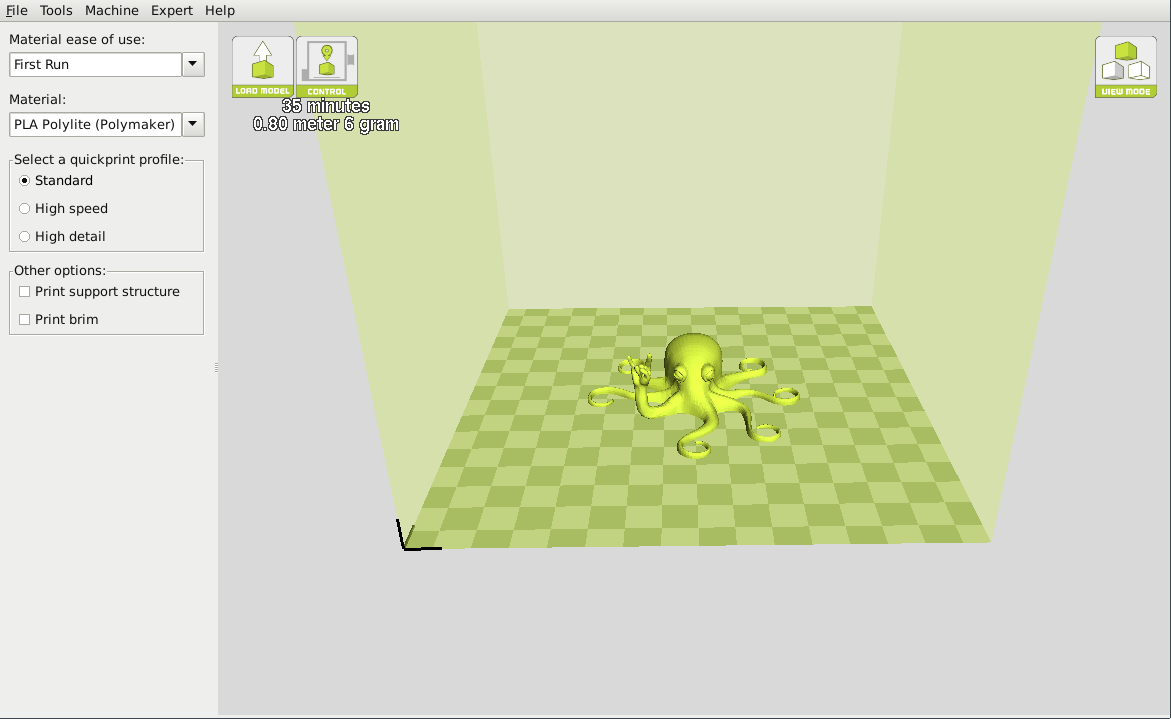
\includegraphics[keepaspectratio=true,angle=0,height=0.4\textheight,width=1.0\textwidth]{QPscreen.png}
\caption{Quick Print Settings}
\label{fig:Cura}
\end{figure} 
% (photo highlighting profile, material, diameter, and other)
After setting up Cura for the first time, you will be shown the main interface screen. (Fig. \ref{fig:Cura}, page \pageref{fig:Cura}): 

\subsection{\texttt{Material Selection}}
\index{material selection}
\index{filament}
\index{filament vendors}
We have the different filament types separated by \texttt{Material ease of use.} From the \texttt{Material ease of use} drop down, select \texttt{"All"} to view all our pre-loaded filament slicing profiles. The Mini ships with a filament sample for the first print. Refer to the included Quick Start Guide for the proper ``First Run'' settings.

\subsubsection{\texttt{Different Filament Manufacturers}}
Different manufacturers have different formulations for their specific brand. These different formulations may have different ideal settings. We usually use 6kg - 10kg of filament when developing these profile settings. \textcolor{red}{We highly recommend using the filament brands listed in Cura LulzBot Edition. Beautiful 3D printed objects start with reliable and consistent filament.} Our profiles will be good starting points for other manufacturers but they may not be ideal.

\subsection{\texttt{Selecting a Quick Print Profile}}
\index{quick print profile}
\index{resolution}
\index{layer height}
\glossary{Resolution}{In general terms, the resolution you print at can be determined by the layer height you use. The LulzBot Mini can print at a layer heights of 0.05mm to 0.50mm with the standard tool head.}
The print quality settings can be found in the top left-hand corner of the window. For most filaments, there will be \texttt{Standard}, \texttt{High Speed}, and \texttt{High Detail} options. Some of the more exotic filaments may have fewer profiles.

\begin{description}
\item[\texttt{High Detail}] \hfill \\
Designed to give greater detail and finer objects. This will have a smaller layer height, which will make each layer thinner, so that curves seem more natural and walls seem less noticeable. This setting will also require more layers to be laid down, increasing overall print time.
\index{High Detail}

\item[\texttt{Standard}] \hfill \\
Designed to give a balanced resolution, by increasing the layer height and print speeds. This will make the organic curves slightly more step-like than the fine setting, but will reduce printing time.
\index{Standard}

\item[\texttt{High Speed}] \hfill \\
Designed for the fast prints, where overall model finish is not of concern. Most commonly used for quick iteration of designs found in rapid prototyping.
\index{High speed}
\end{description}

\subsection{\texttt{Printing Support Material}}
\index{Support Material}
%%%% Saved for standalone Cura Manual %%%%
%The TAZ and Mini are able to print models that have angles and overhangs, even without support material depending on the overhang distance and angle. Turn this option on if your model could benefit from support material.
The LulzBot Mini 3D printer is able to print models that have angles and overhangs, even without support material depending on the overhang distance and angle. Turn this option on if sections of your model are being are extending in mid air. This will build up material underneath the portion extending in mid air, preventing gravity from making it droop.
%The LulzBot TAZ 3D printer is able to print models that have angles and overhangs, even without support material. This will depend on the overhang distance and angle of your particular model file. Turn this option on if sections of your model are being are extending in mid air. This will build up material underneath the portion extending in mid air, preventing gravity from making it droop.

\subsection{\texttt{Brim}}
\index{Brim}
Brim is used to increase surface area of the part you're printing, thereby ensuring proper part adhesion. This will print a single layer high edge around the base of the part, helping first layer adhesion and minimizing warping.

\subsection{\texttt{Load Model File}}
\index{Load Model}
\index{load model}
\index{3D models}
\index{STL}
\index{OBL}
\index{AMF}
Select the 3D model you would like to print. Either use the \texttt{Load Model} button or select \texttt{File} > \texttt{Load Model}. Once the file has been loaded, you will see a 3D rendering of your object on the build platform. Select the model to see the various options. 

\subsection{\texttt{Model Orientation}}
\index{orientation}
Move your model to change where it is printed on the build plate. Do this by left clicking on the model and dragging it to the desired location. The \texttt{black} outlined corner of the 3D print bed view represents the front left hand corner of the build plate on your printer. You can view your model from different angles by holding down the right mouse button and dragging. %Not sure if this last sentence should be reworked or put in a separate section.
\begin{figure}[H]
\centering
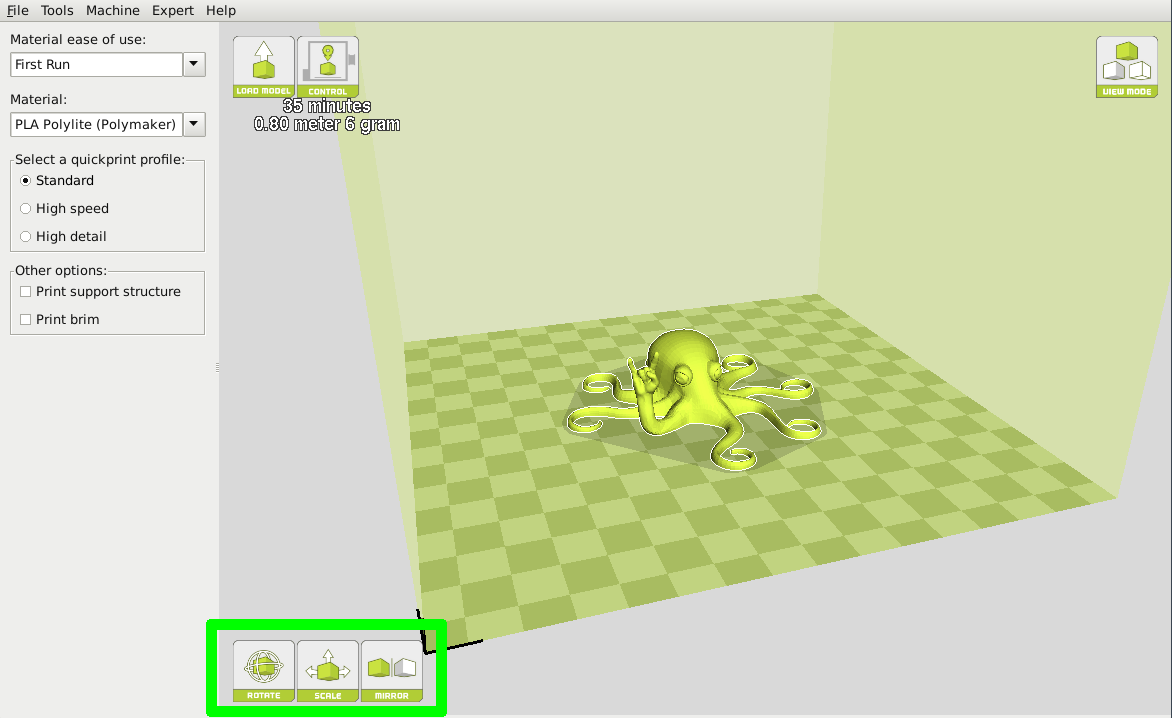
\includegraphics[keepaspectratio=true,angle=0,height=0.4\textheight,width=1.0\textwidth]{optionsRSM1.png}
\caption{Options after selecting model}
\label{fig:Orientation}
\end{figure}

\subsubsection{\texttt{Rotate}}
\index{Rotating Model File}
%%%% Alternate explanation %%%%
%The \texttt{Rotate} button will give you the ability orient your model in along all three axes. Once you click the rotate button, three circles will surround your model. The red circle will allow you to rotate in the XY plane. The Yellow circle will rotate in the XZ plane. The Green circle will rotate in the YZ plane.
\definecolor{yellow1}{cmyk}{0,0,1,0.30}
\definecolor{green1}{rgb}{0.30,1,0.30}
The \texttt{Rotate} button will give you the ability to orient your model in along all three axes. Once you click the rotate button, three circles will surround your model. The \textcolor{red}{red circle} will allow you to rotate around the \textcolor{red}{Z-axis}. The \textcolor{yellow1}{Yellow circle} will rotate around the \textcolor{yellow1}{Y-axis}. The \textcolor{green}{Green circle} will rotate around the \textcolor{green}{X-axis}. Cura defaults to 15 degree increments. Hold \texttt{Shift} to rotate by \texttt{One Degree Increments}. (Fig. \ref{fig:Rotating your Model}, page \pageref{fig:Rotating your Model})

\begin{figure}[H]
\centering
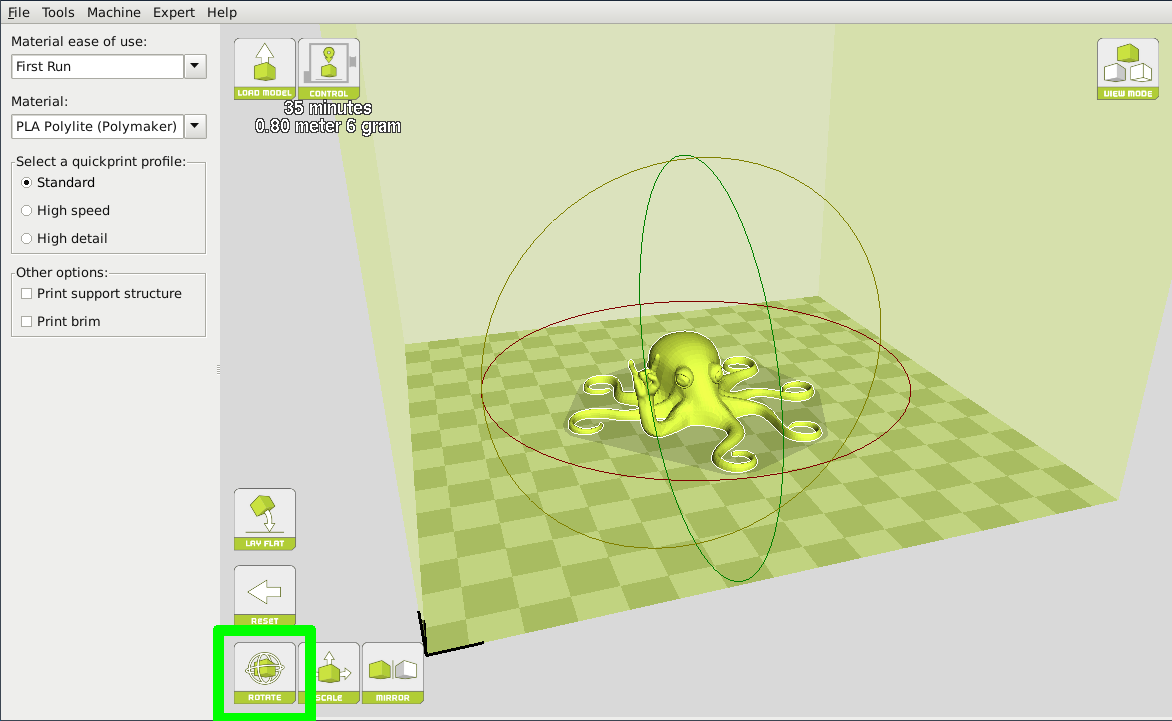
\includegraphics[keepaspectratio=true,angle=0,height=0.4\textheight,width=1.0\textwidth]{rotateoptions.png}
\caption{Rotating your Model}
\label{fig:Rotating your Model}
\end{figure}

\subsubsection{\texttt{Lay Flat}}
The \texttt{Lay Flat} button will ensure that the flat portion of your print is securely attached to the bed. It is highly recommended to use this option after rotating your model in the Z direction, as it will help prevent potential adhesion issues during the print.
%\begin{figure}[hbt]
%\centering
%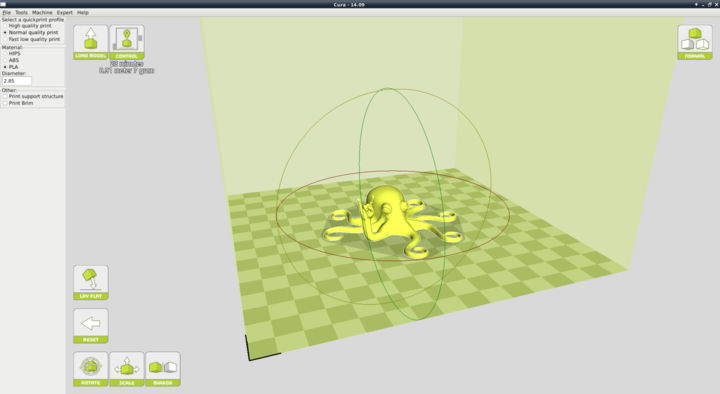
\includegraphics[keepaspectratio=true,angle=0,height=0.4\textheight,width=1.0\textwidth]{Rotate.png}
%\caption{Rotating your Model}
%\label{fig:Rotating your Model}
%\end{figure}

\subsubsection{\texttt{Reset}}
The \texttt{Reset} button will return your model to the original orientation as defined by the CAD program used to create the model.
%\begin{figure}[hbt]
%\centering
%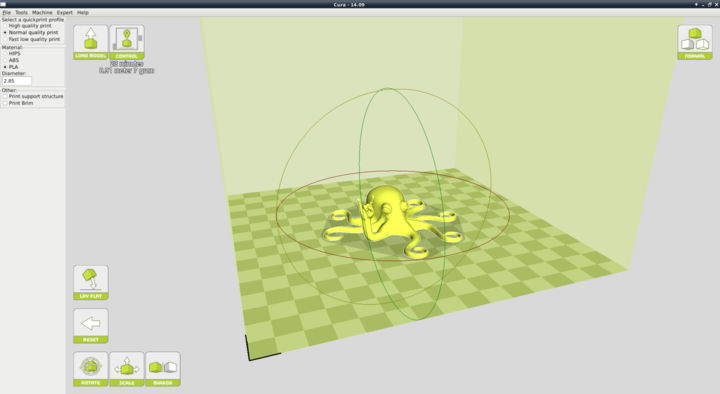
\includegraphics[keepaspectratio=true,angle=0,height=0.4\textheight,width=1.0\textwidth]{Rotate.png}
%\caption{Rotating your Model}
%\label{fig:Rotating your Model}
%\end{figure}

\subsubsection{\texttt{Scale}}
The \texttt{Scale} button displays the model dimensions, along with the ability to scale along the X Y or Z axes. Anything \texttt{below} the number \texttt{1.0} will reduce the objects size, while anything \texttt{above} the number \texttt{1.0} will increase the objects size. As a default, it will be set to uniform scaling. This will cause the X Y and Z axes to be scaled by the same amount when you make a change to any of them. To disable this, select the lock in the lower section of the scaling window. 
\begin{figure}[H]
\centering
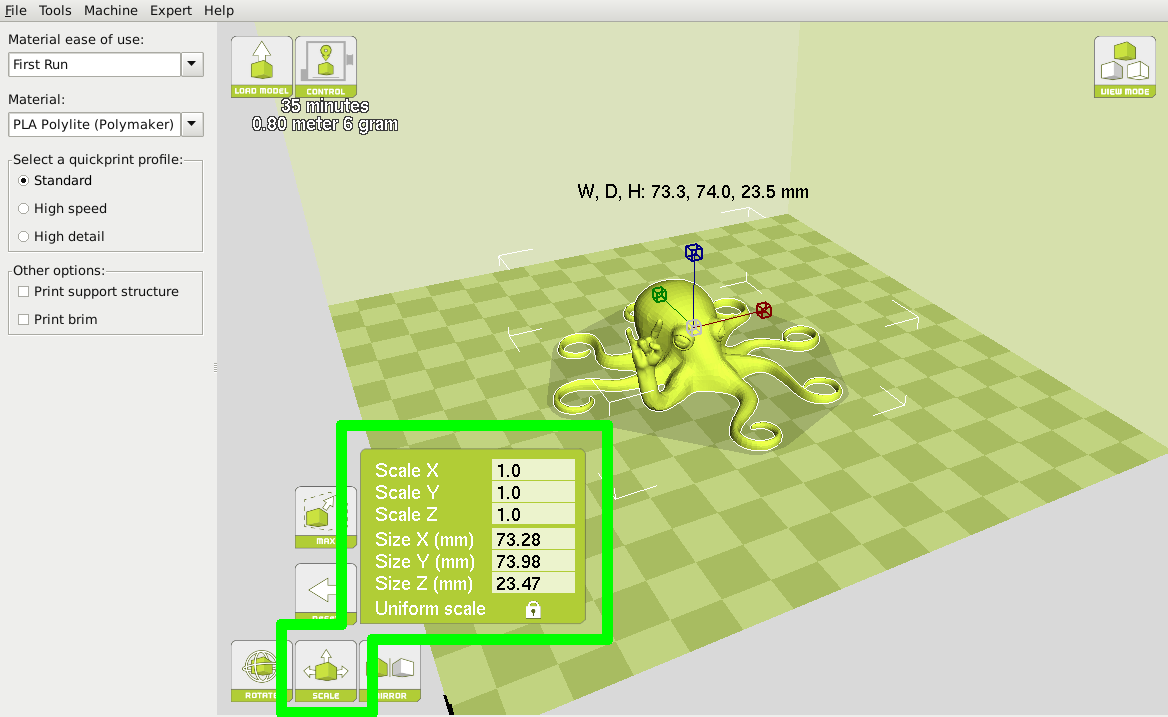
\includegraphics[keepaspectratio=true,angle=0,height=0.4\textheight,width=1.0\textwidth]{scaleoptions.png}
\caption{Scaling your Model}
\label{fig:Scaling your Model}
\end{figure}

\section{\texttt{View Options}}
\index{View Options}
Different modes allow you to view your model in a variety of ways. This can be helpful for spotting issues before the print even starts. 

\subsection{\texttt{Normal}}
\index{normal view}
This is the standard view and shows the solid outer surfaces of the model. (Fig. \ref{fig:Normal View}, page \pageref{fig:Normal View}): 

\begin{figure}[H]
\centering
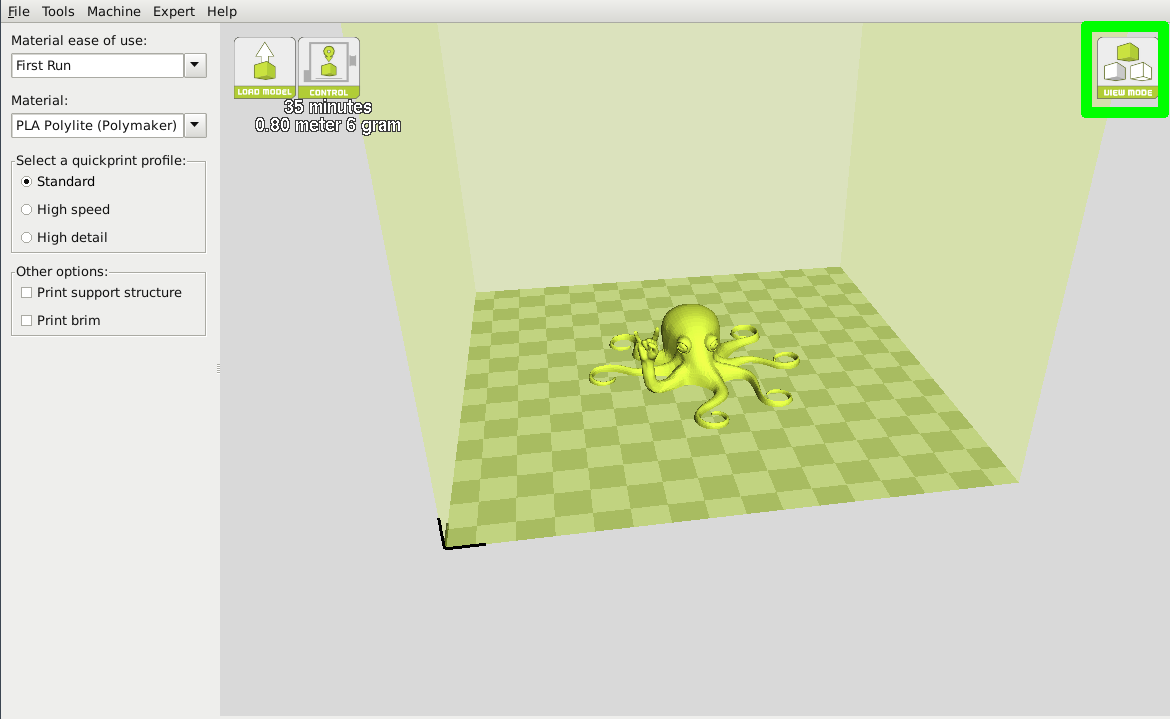
\includegraphics[keepaspectratio=true,angle=0,height=0.3\textheight,width=1.0\textwidth]{normalview.png}
\caption{View in Normal Mode}
\label{fig:Normal View}
\end{figure}

\subsection{\texttt{Overhang}}
\index{Overhang View} 
Overhang mode shows where your model may need support material. In Fig. \ref{fig:Overhang_View}, page \pageref{fig:Overhang_View} the red highlighted areas show overhangs and more severe angles and areas where support material is recommended. The overhang threshold can be defined in Expert Settings. 
\begin{figure}[H]
\centering
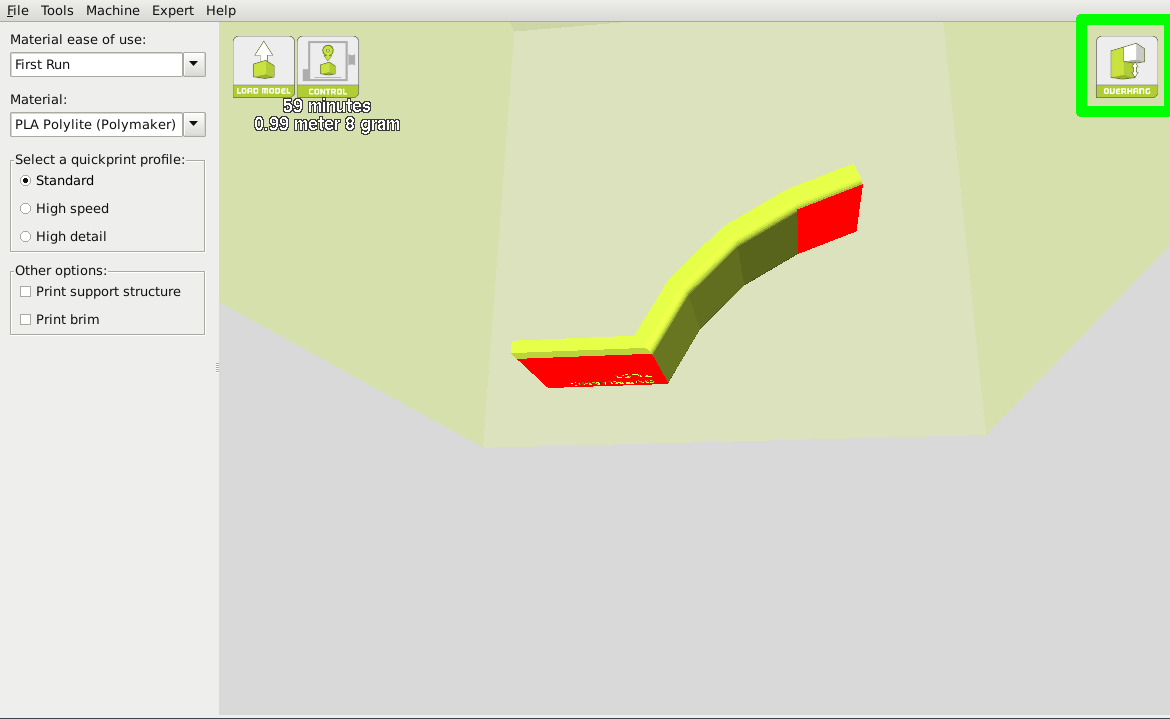
\includegraphics[keepaspectratio=true,angle=0,height=0.3\textheight,width=1.0\textwidth]{overhangview.png}
\caption{View in Overhang}
\label{fig:Overhang_View}
\end{figure}

\subsection{\texttt{Ghost}}
\index{Ghost View}
Ghost view mode makes the model translucent to allow you to see what is behind it.
\begin{figure}[H]
\centering
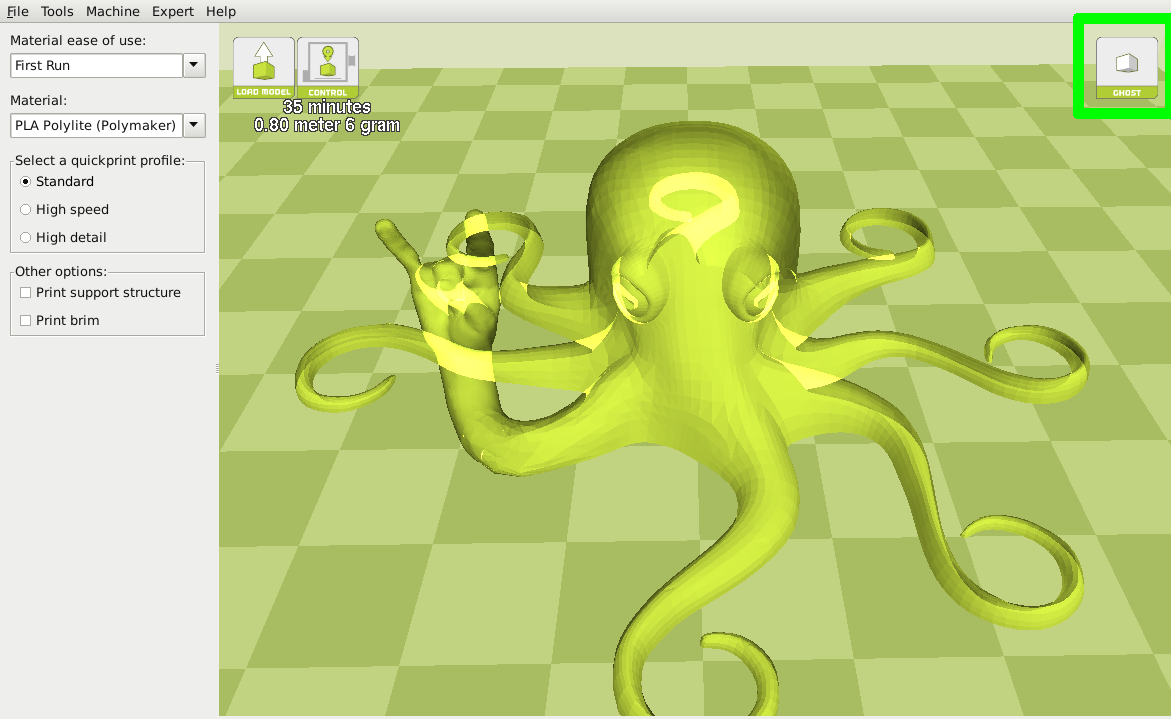
\includegraphics[keepaspectratio=true,angle=0,height=0.3\textheight,width=1.0\textwidth]{ghostview.png}
\caption{View in Ghost}
\label{fig:Ghost View}
\end{figure}

\subsection{\texttt{Xray}}
\index{X-ray View}
X-ray allows you to look inside of the object. This is helpful for detecting any manifold errors or other possible issues with your model. Problem areas will be highlighted in red. (Fig. \ref{fig:Xray View}, page \pageref{fig:Xray View})
\begin{figure}[H]
\centering
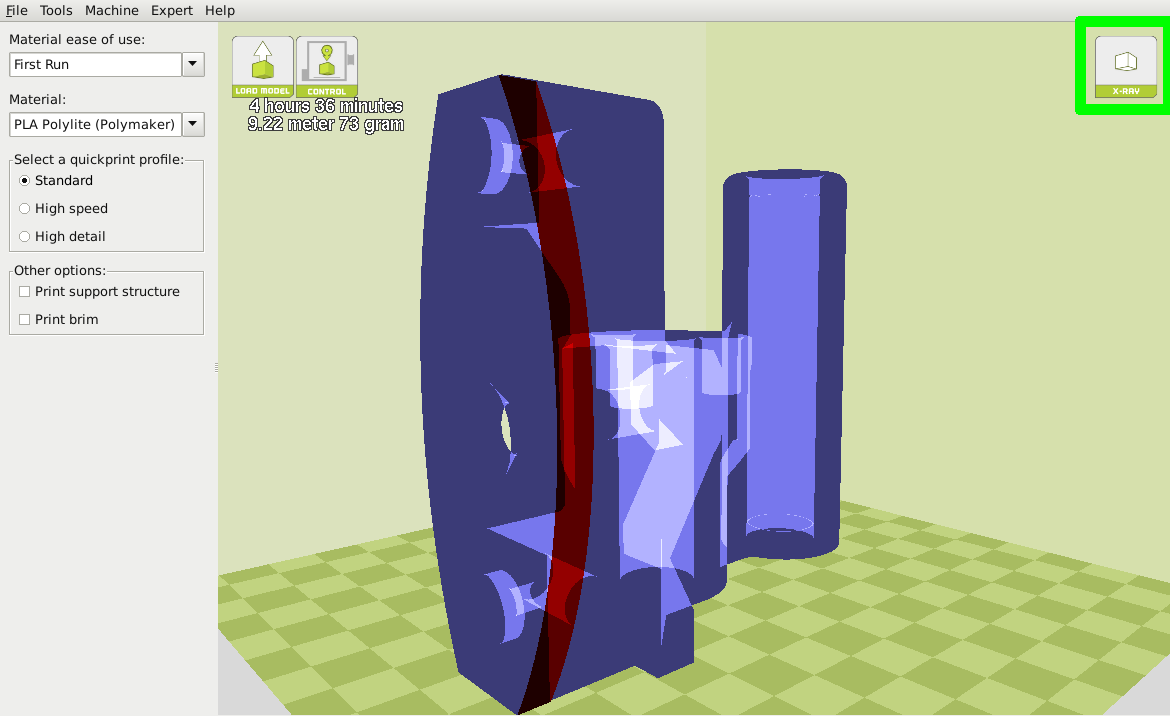
\includegraphics[keepaspectratio=true,angle=0,height=0.3\textheight,width=1.0\textwidth]{xrayview.png}
\caption{View in Xray}
\label{fig:Xray View}
\end{figure}

\subsection{\texttt{Layers}}
\index{layers view}
To view the tool path of your print head and to ensure no skipped layers or gaps use this option. Use the slide bar on the right hand side of the window to move up and down through the tool path layers. Click the icon below it to view an individual layer at a time. If the \texttt{Print support structure} option is activated in Cura, support structure will be shown in blue.
\begin{figure}[H]
\centering
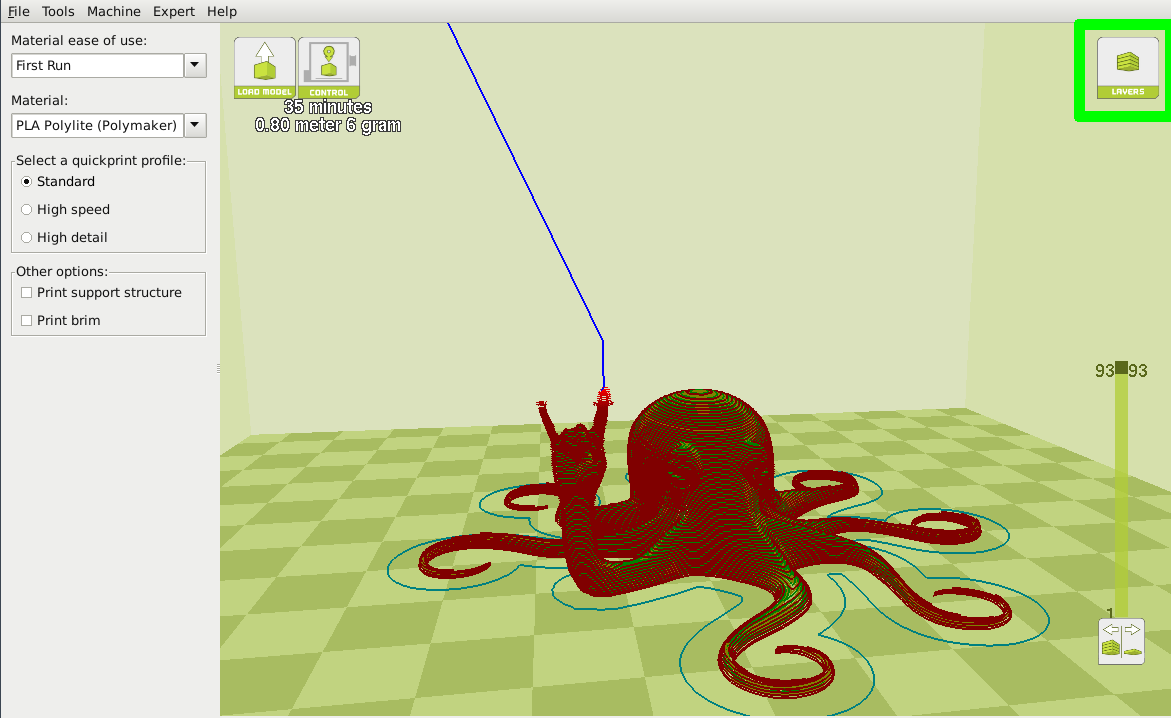
\includegraphics[keepaspectratio=true,angle=0,height=0.3\textheight,width=1.0\textwidth]{layers1.png}
\caption{View in Layers}
\label{fig:Layers View}
\end{figure}

\begin{figure}[H]
\centering
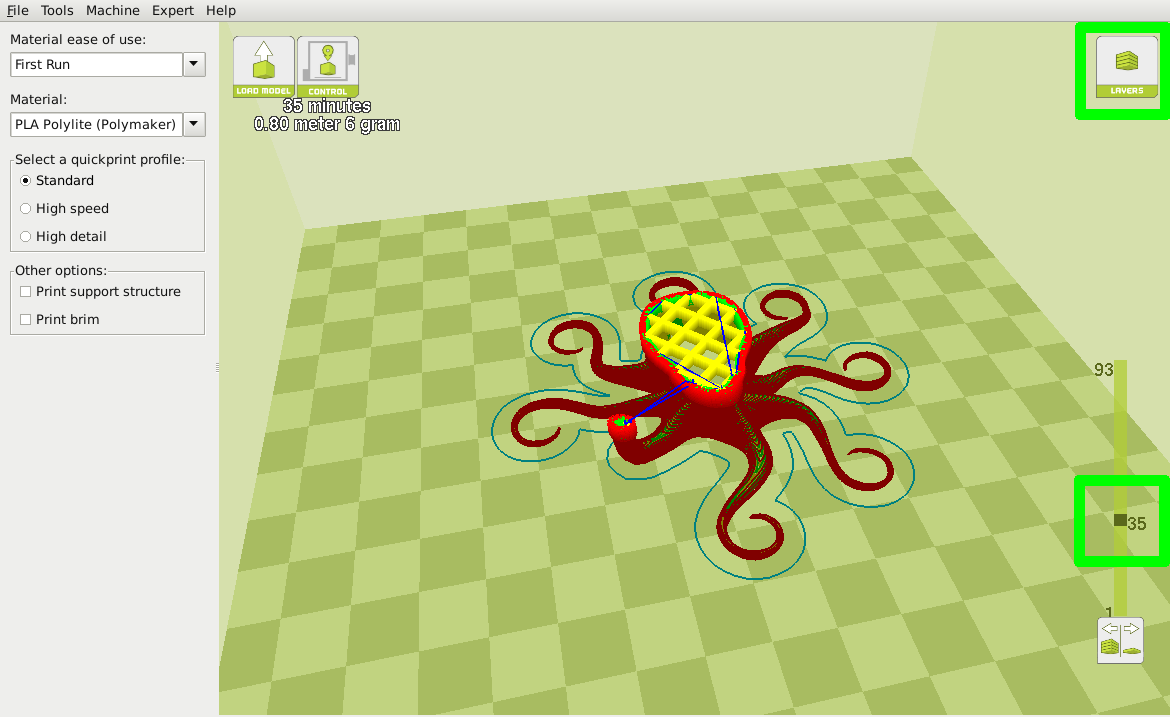
\includegraphics[keepaspectratio=true,angle=0,height=0.3\textheight,width=1.0\textwidth]{layers2.png}
\caption{Viewing Cumulative Layers}
\label{fig:Mid Layers View}
\end{figure}

\begin{figure}[H]
\centering
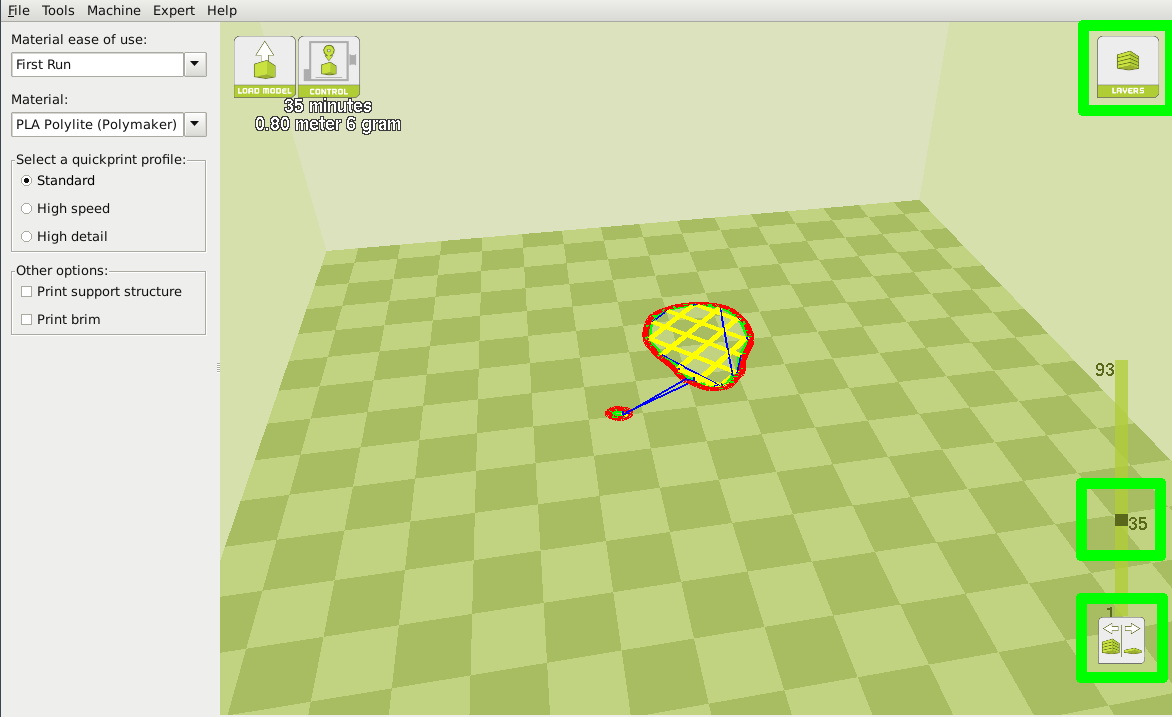
\includegraphics[keepaspectratio=true,angle=0,height=0.3\textheight,width=1.0\textwidth]{layers3.png}
\caption{Viewing An Individual Layer}
\label{fig:Specific Layer}
\end{figure}


\section{\texttt{Starting Your First Print}}
\index{First Print}
Once you have your model, profile, and filament loaded, it is time for your first print! Refer to the \texttt{Quick Start Guide} included with your 3D printer. A PDF version is available at \texttt{LulzBot.com/downloads}.

\begin{comment} %%%% Turn the following on for standalone Cura manual %%%%
\subsection{Mini}

Select the \texttt{Print/Control} option in the top left hand corner of your build volume. This will bring up your Pronterface user interface. Please wait for the window to state \texttt{operational} before sending any commands to the printer.

%\pageref{fig:Print Control}).
\begin{figure}[hbt]
\centering
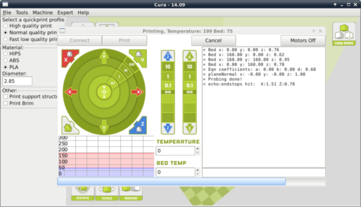
\includegraphics[keepaspectratio=true,angle=0,height=0.4\textheight,width=1.0\textwidth]{print_control.png}
\caption{Print Control Screen}
\label{fig:Print Control}
\end{figure}

\subsection{\texttt{Pausing Mid-Print}}
\index{pausing the printing process}
\index{pause print}
You will notice after you click the print button through Cura, it will change to a pause button. When activated, it will pause the print and automatically move your print head away from your object. This will allow color changes or material changes mid print.

\subsection{\texttt{Automatic Bed Leveling}}
\index{automatic bed leveling}
\index{ABL}
Before each print your Mini will go through a wiping and a probing procedure in order to determine the slope/tilt of your bed. If your nozzle is dirty or not cleaned properly, this will prevent the printer from being able to create an electrical contact with the corners. Your Mini will automatically retry the wiping and probing procedure if this happens, up to a maximum of three times. If three consecutive wipes and probes have failed, the printer will stop and a warning will sound. If this is happening consistently, you should replace the wiping pad and/or adjust your wiping and probing temps for that specific filament. See section \ref{sssec:num1} on page \pageref{sssec:num1} for details on changing these temps.
%\subsection{Mini}

%Select the \texttt{Print/Control} option in the top left hand corner of your build volume. This will bring up your Printer Interface. Please wait for the window title to display \texttt{operational} before sending any commands to the printer..

%\pageref{fig:Print Control}).
%\begin{figure}[hbt]
%\centering
%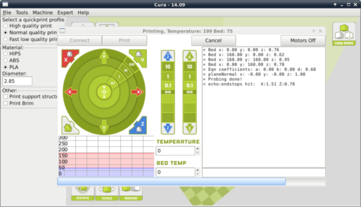
\includegraphics[keepaspectratio=true,angle=0,height=0.4\textheight,width=1.0\textwidth]{print_control.png}
%\caption{Print Control Screen}
%\label{fig:Print Control}
%\end{figure}

%\subsection{TAZ}

%Your TAZ 3D printer has the ability to print directly from a computer using the included USB cable, or directly from the SD card by using the Graphical LCD controller.


\begin{comment}
%%%% SD Printing %%%%
\subsection{\texttt{Printing from SD Card}}
\index{graphical LCD controller}
\index{GLCD}
\index{tetherless printing}

Load your model into Cura with the proper filament and profile selected. Next, insert the included SD card into your computer. Select \texttt{File} > \texttt{Save GCODE} and choose the SD card location to save your GCODE file to your SD card. Safely eject the card from the computer, and insert it into the Graphical LCD Controller. 

%\subsection{\texttt{Set Temperature}}

%Turn on the heated bed and hot end by using the Graphical LCD controller and navigating to: \texttt{Temperature} > \texttt{Select Filament type}. If you are using other than a preset material, you can set your desired temperatures by going to \texttt{Temperature} > \texttt{Custom Temp} > \texttt{Nozzle/Bed}. Wait for your 3D printer to reach specified temperatures.

\subsection{\texttt{Start Print}}
Thanks to the TAZ automatic bed leveling system, it is now time to kick off the print! Through the LCD screen go to: \texttt{Print From SD} > \texttt{Desired File}. Your TAZ will then go through it's automatic cleaning and wiping process before starting the print. This should take approximately 5 minutes.

\end{comment}

%%%% Tethered printing %%%%

%\pageref{fig:Print Control}).

\begin{figure}[H]
\centering
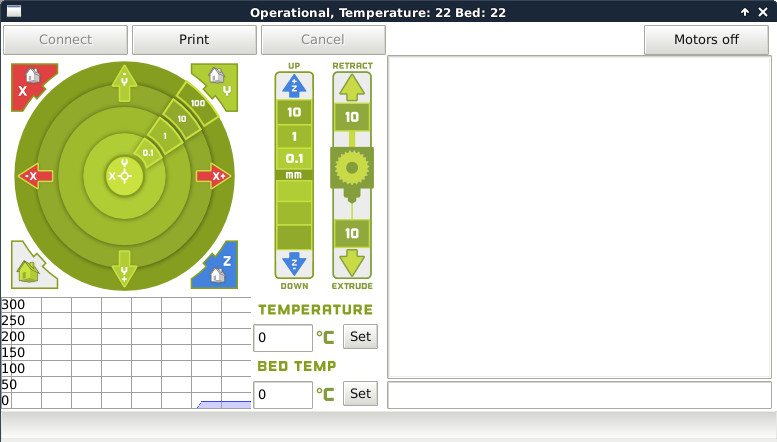
\includegraphics[keepaspectratio=true,angle=0,height=0.4\textheight,width=1.0\textwidth]{ControlBox17.1.jpg}
\caption{Control Screen}
\label{fig:Control}
\end{figure}
\subsection{\texttt{Pausing Mid-Print}}
\index{pausing in the printing process}
\index{pause print}
You will notice after you click the print button through Cura, it will change to a pause button. When activated, it will pause your print and automatically move your print head away from your object. This will allow color changes or material changes mid print.

\subsection{\texttt{Automatic Bed Leveling}}
\index{Automatic Bed Leveling}
\index{ABL}
Before each print your Mini will go through a wiping and a probing procedure in order to determine the slope/tilt of your bed. If your nozzle is dirty or not cleaned properly, this will prevent the printer from being able to create an electrical contact with the corners. Your Mini will automatically retry the wiping and probing procedure if this happens, up to a maximum of three times. If three consecutive wipes and probes have failed, the printer will stop and a warning will sound. \textcolor{red}{If your Mini does not re-wipe after a failed probe, update your firmware.} Directions for updating firmware can be found in section \ref{ssec:num2} on page \pageref{ssec:num2}. If probe failures are happening consistently, you should replace the wiping pad and/or adjust your wiping and probing temps for that specific filament. See section \ref{sssec:num1} on page \pageref{sssec:num1} for details on changing these temps. %reference updating firmware section once created in advanced or maintenanceQP

\subsection{\texttt{Recommended Temperatures}}
\index{Temperatures}
Different filaments have different ideal temperatures for extrusion, bed adhesion, and part removal. Your LulzBot Mini will have these automatically set when using our recommended profiles. We have found that for certain materials a glue stick is required for successful bed adhesion and/or part release. Glue stick can also be added to help first layer adhesion on any material, and may be helpful for objects with a larger surface area. 
\begin{table}[H]
	\begin{center}
 		\hspace*{-1.5cm}\begin{tabular}{||c c c c c||} 
 		\hline
 		Filament Type & Bed Preparation & Nozzle Temp & Bed Temp & Removal Temp \\ [0.5ex] 
 		\hline\hline
 		ABS & Clean PEI & 230-250 & 110 & 50 \\ 
 		\hline
 		PLA & Clean PEI & 195-215 & 60 & 45\\
 		\hline
 		HIPS & Clean PEI & 230-250 & 110 & 50 \\
 		\hline
 		Laywoo-D3 & Clean PEI & 175-195 & 60 & 45 \\
 		\hline
		bambooFill & Clean PEI & 185-195 & 60 & 50 \\ 
 		\hline
		woodFill & Clean PEI & 185-195 & 60 & 50 \\
 		\hline
 		Laybrick & Clean PEI & 175-195 & 60 & 45 \\
		\hline
		bronzeFill & Clean PEI & 225-235 & 60 & 50 \\
		\hline
		copperFill & Clean PEI & 225-235 & 60 & 50 \\
 		\hline 
 		Magnetic Iron PLA & Clean PEI & 220-230 & 60 & 50 \\
 		\hline
 		Stainless Steel PLA & Clean PEI & 220-230 & 60 & 50 \\
 		\hline
 		Conductive PLA & Clean PEI & 215-230 & 60 & 50 \\
		\hline
		High Temp PLA & Clean PEI & 220-230 & 60 & 40 \\
 		\hline
 		nGen & Glue stick & 220-240 & 85 & 60 \\
 		\hline
 		t-glase & Glue stick & 240-260 & 60 & 45 \\
 		\hline
 		Flexible Filaments & Glue stick & 215-230 & 50 & 35 \\  
 		\hline
 		Nylons & Glue stick & 220-270 & 110 & 50 \\
 		\hline
 		Polycarbonate & Glue stick & 260-300 & 110 & 50 \\ 
 		\hline
 		Polycarbonate + ABS & Glue stick & 260-280 & 110 & 50 \\
 		\hline
 		INOVA 1800 & Glue stick & 235-255 & 75 & 50 \\
 		\hline
 		n-vent & Glue stick & 225-245 & 60 & 50 \\
 		\hline
  		PVA & Glue stick & 180-200 & 60 & 45 \\
 		\hline
 		PC-Max & Glue stick & 240-270 & 100 & 50 \\
 		\hline
 		colorFabb_HT & Glue stick & 260-280 & 110 & 50 \\ [1ex]
 		\hline
		\end{tabular}
		\caption{Recommended Temperatures}\label{tab:a}
	\end{center}
\end{table}
%%mini:
%This will start the printing process: (set the appropriate temperatures, go through the automatic bed leveling procedure, and start printing your model).
%\pageref{fig:Print Control}).


\section{\texttt{Removing Your First Print}}
\index{Removing a Print}
After your first print has finished, you need to wait for the part to cool down.  Your parts will be easier to remove if you allow your heated bed to cool down to optimal temperature. This will allow the plastic to contract, making it easier to remove. \texttt{The Y-axis will move forward once it reaches the ideal print removal temperature.}

Once your heated bed has cooled, use the blue handled knife that was included with your toolkit to remove the item. Carefully insert the blade of the knife between your print and heated bed. Once underneath the part rotate the blade- lifting with the sharp edge into the part, to gently pop the piece off your plate.
%\begin{figure}[hbt]
%\centering
%\includegraphics[keepaspectratio=true,angle=0,height=0.4\textheight,width=1.0\textwidth]{remove_part.png} %%%% Photo needed %%%%
%\caption{Remove Part}
%\label{fig:Remove part}
%\end{figure}

\section{\texttt{Full Settings}}
\index{Full Settings}
When you first switch to Full Settings, Cura will need to know what filament, manufacturer, and quality you wish to use. It will automatically transfer our quickprint settings over to allow adjustments if one is selected. \textcolor{red}{IF A QUICKPRINT PROFILE IS NOT AVAILABLE, YOU WILL NEED TO MANUALLY LOAD ONE.} We recommend using our tested profiles that are available here: \texttt{LulzBot.com/Cura}. You will want to choose the profile that matches your filament and quality needs. Once downloaded, you can load the file into Cura by selecting \texttt{File} > \texttt{Open Profile}. This will automatically update all of your Cura settings for use with your specific filament.
\begin{figure}[H]
\centering
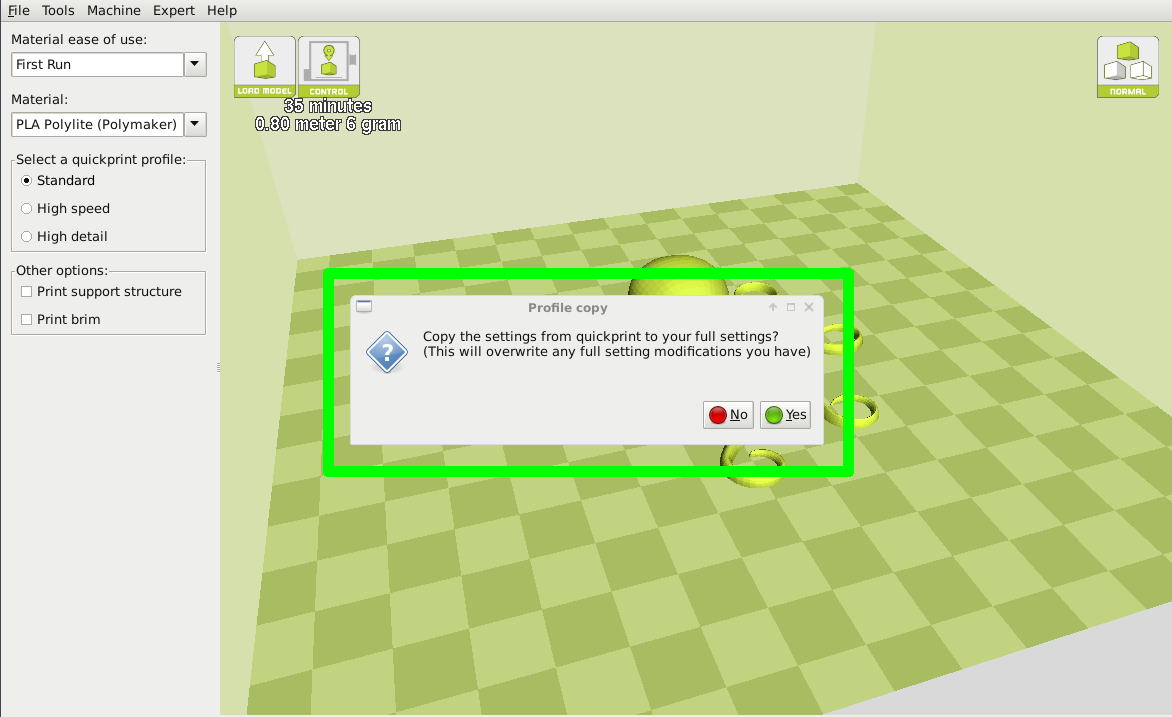
\includegraphics[keepaspectratio=true,angle=0,height=0.4\textheight,width=1.0\textwidth]{copyprofile.png}
\caption{Transferring a Profile}
\label{fig:Transferring a Profile}
\end{figure}
Once the switch has been made to full settings, you will now have access to a wide variety of options. You will notice 4 new tabs: \texttt{Basic, Advanced, Plugins, Start/End-Gcode}. In the following sections we will describe each option, and how they will affect your prints.
\begin{figure}[H]
\centering
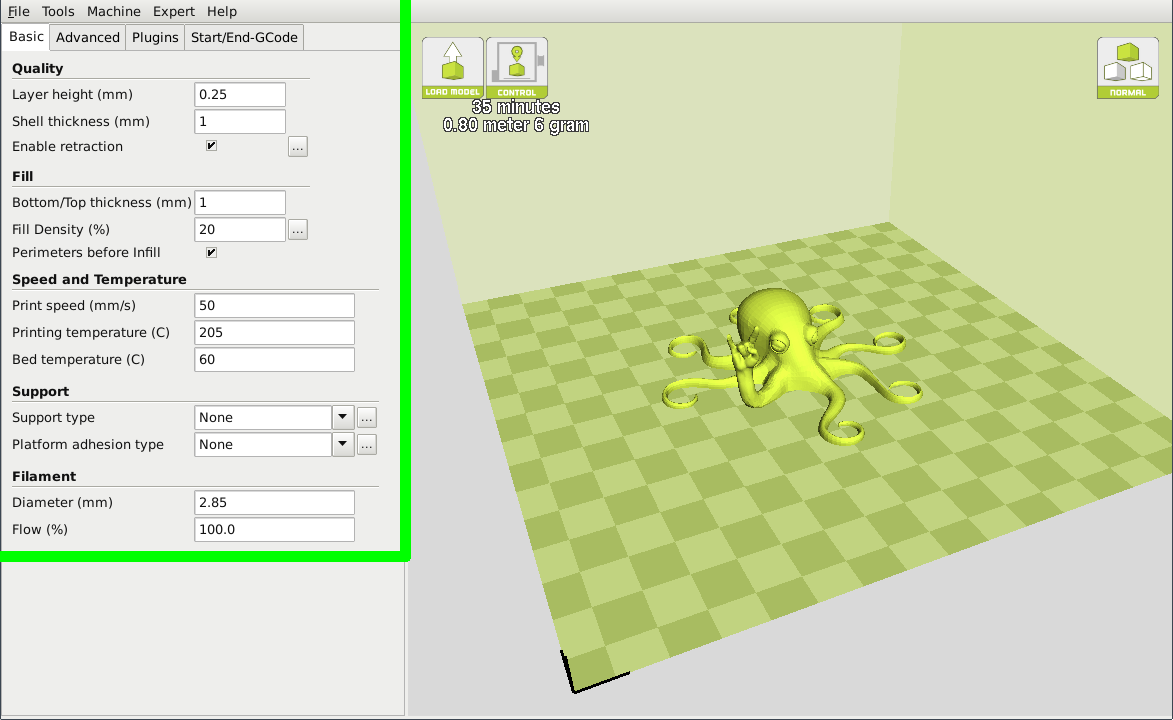
\includegraphics[keepaspectratio=true,angle=0,height=0.4\textheight,width=1.0\textwidth]{fullsettings.png}
\caption{View in Full Settings}
\label{fig:View in Full Settings}
\end{figure}

%\subsection{\texttt{Loading a Profile}}
%\index{Loading Profile}
%Profiles determine how Cura turns your STL file into Gcode that controls your printer. Different filaments require different settings for optimal performance. As new filaments are being developed every day, there may be a time you need to manually load a profile. You can download our recommend profiles at: \texttt{https://www.lulzbot.com/support/mini-cura-profiles}. Once downloaded, load the filament specific .ini file by going to \texttt{File > Open Profile}.
%\begin{figure}[hbt]
%\centering
%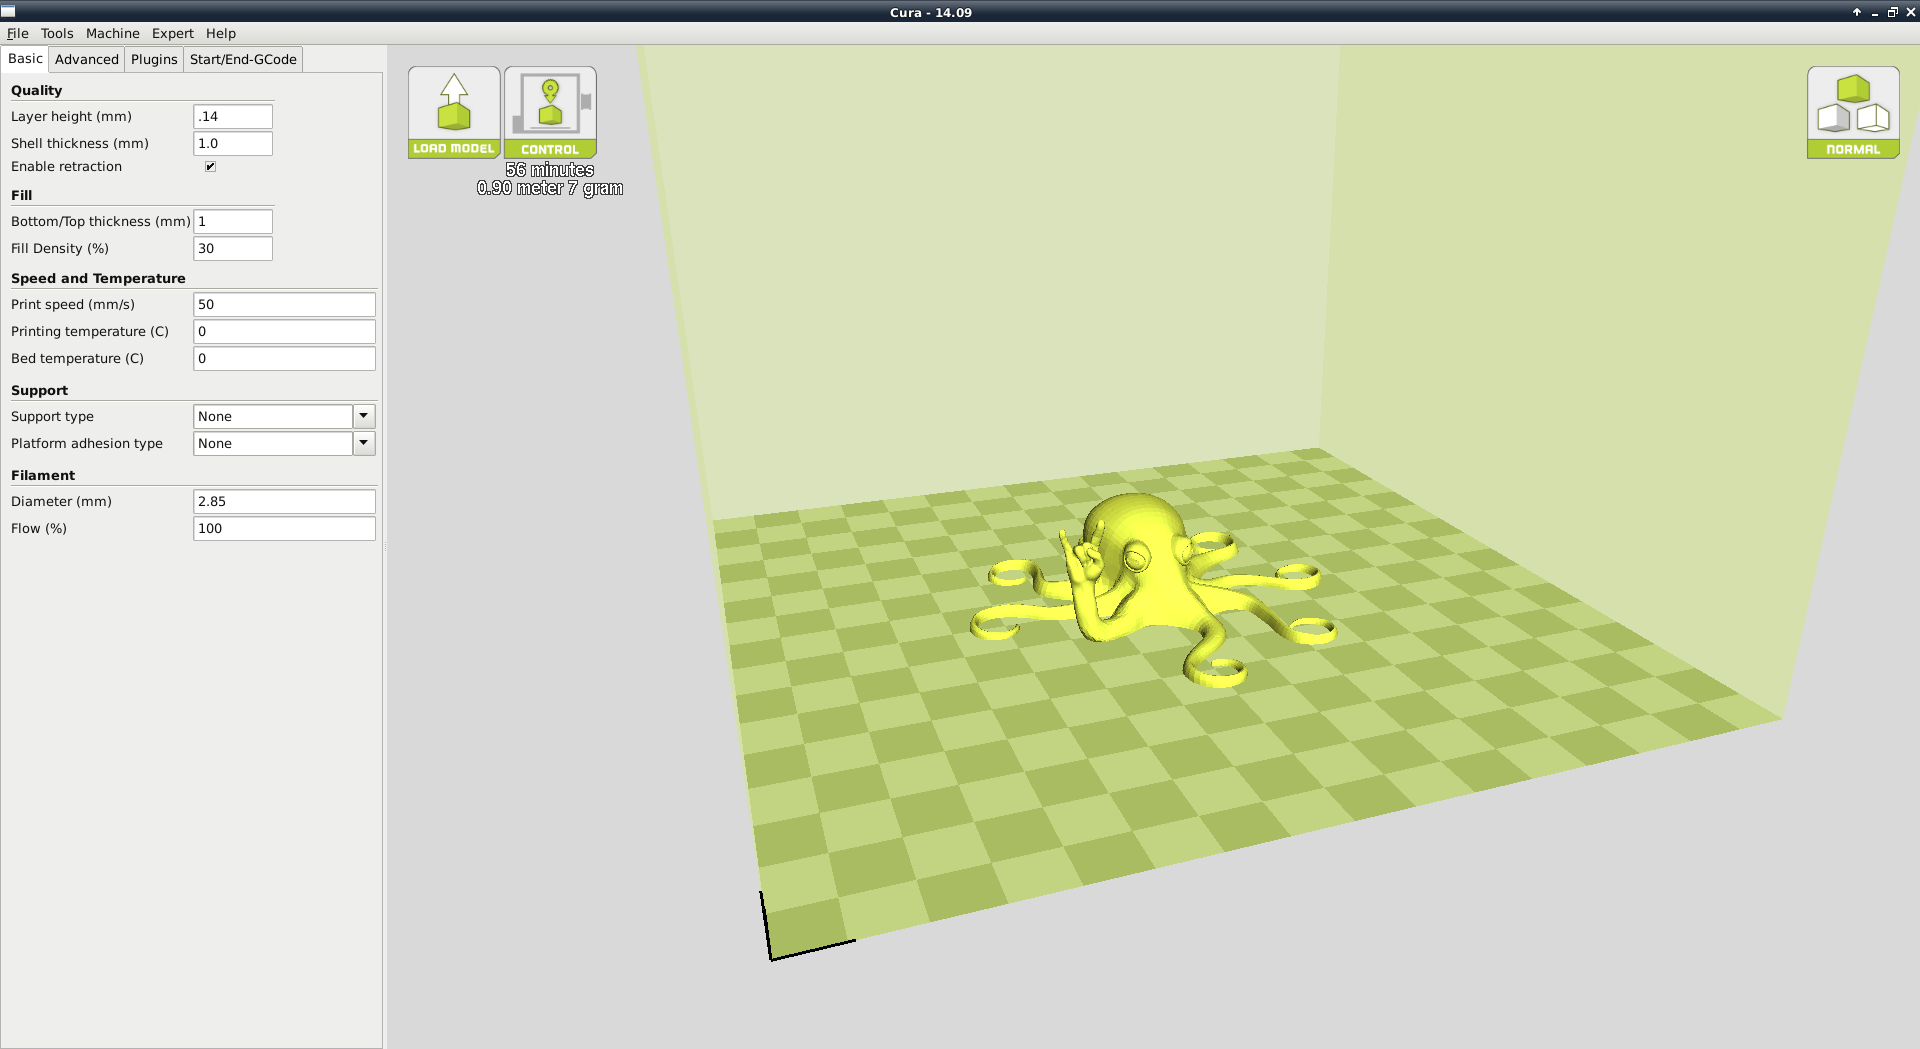
\includegraphics[keepaspectratio=true,angle=0,height=0.4\textheight,width=1.0\textwidth]{Expert.png}
%\caption{View in Full Settings}
%\label{fig:Full Settings View}
%\end{figure}

\section{\texttt{Basic Tab Options}}
\index{Basic Options}

\subsubsection{\texttt{Layer Height}}
\index{Layer Height}
The thickness of each printed layer is known as the ``Layer Height''. The smaller the layer height, the smoother curves will appear. Larger layer heights are better for bridging and overhangs. Smaller layer heights will also increase print time, as it will take more layers to complete the object.
% (Layer height comparison photos)
\begin{figure}[H]
\centering
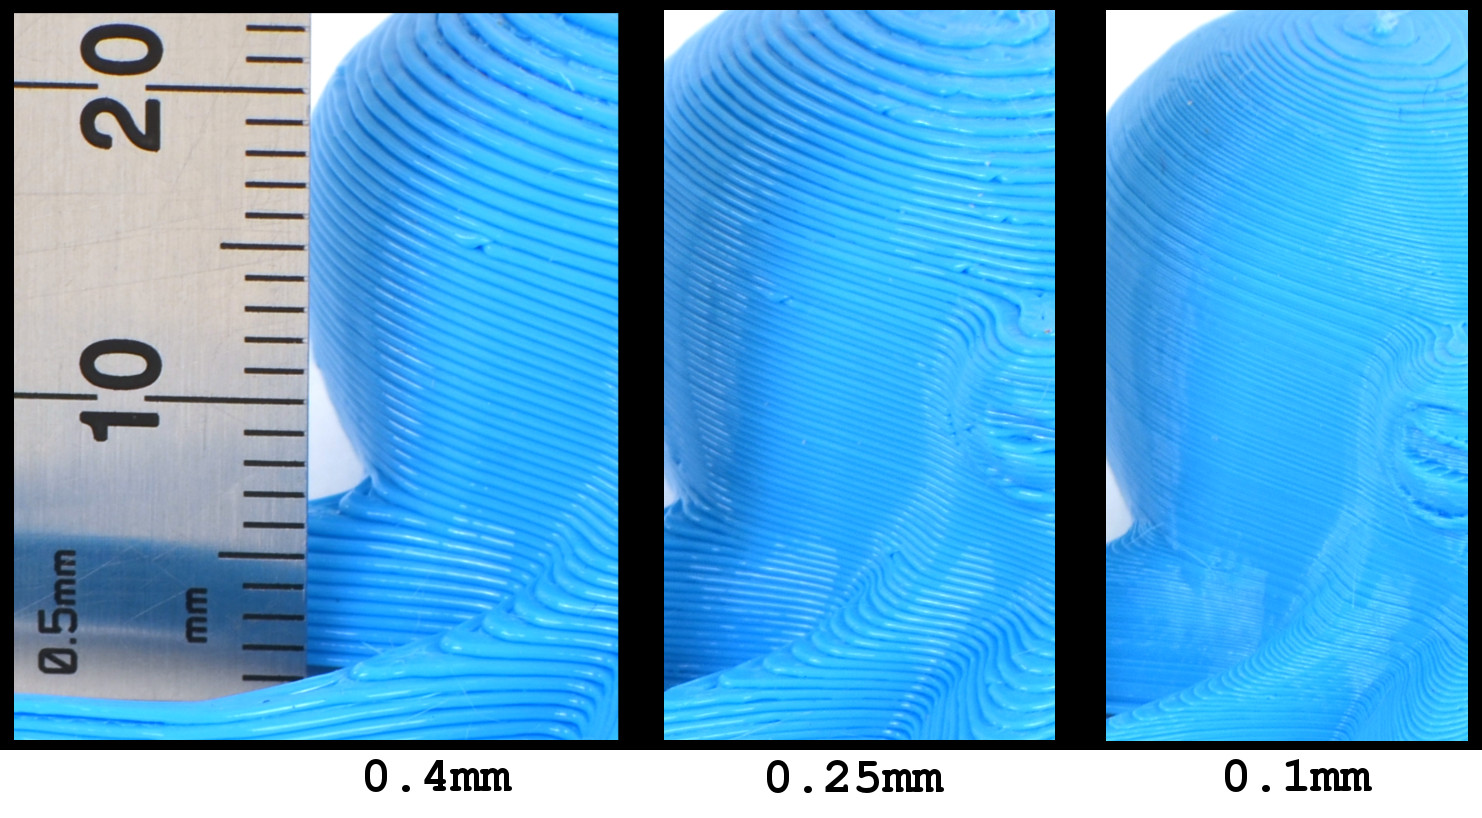
\includegraphics[keepaspectratio=true,angle=0,height=0.4\textheight,width=1.0\textwidth]{ManualLayerHeight.jpg}
\caption{Differences in Layer Height}
\label{fig:Differences in Layer Height}
\end{figure}


\subsubsection{\texttt{Shell Thickness}}
\index{Shell Thickness}
This defines the number of vertical walls that comprise the outside of your model. We recommend keeping this set to multiples of your nozzle width. Your LulzBot Mini 3D printer is equipped with a 0.5mm nozzle. A setting of 1.0mm or 1.5mm is a sufficient for most prints.

\subsubsection{\texttt{Enable Retraction}}
\index{Retraction}
Retraction tells your printer to pull filament out of the hot end upon travel moves. Travel moves are when your print head moves from one area of the print, to another without laying down filament. We recommend keeping this on for all filament types, and adjusting the retraction length and speed for the specific filament.
%(Details given in advanced tab section. ((Reference?))

\subsubsection{\texttt{Bottom/Top Thickness (mm)}}
\index{Bottom Thickness}
\index{Top Thickness}
Also known as ``Surface Layers'' this will determine how thick the top and bottom layers are. A larger number here will create a thicker top and bottom which can be helpful for strength, bridging, and quality purposes. We recommend keeping this number as a multiple of your layer height.

\subsubsection{\texttt{Fill Density}}
\index{Fill Density}
This number is expressed as a percentage. 0\% will give a completely hollow print, while 100\% will give you a completely solid object. We have found that 20\% to 40\% fill density is functional for most prints.

\subsubsection{\texttt{Perimeters Before Infill}}
This option will toggle the order in which the infill and perimeters will be printed. We recommend leaving this on.

\subsubsection{\texttt{Print Speed (mm/s)}}
\index{Print Speed}
Your overall printing speed can be adjusted here. This setting will be overridden in certain parts of the print based upon your Advanced Speed Settings. If no speeds are determined in the advanced settings tab, your printer will default to this setting. %See Advanced Section \ref{sssec:Travel Speed}, page \pageref{sssec:Travel Speed} 


\subsubsection{\texttt{Printing Temperature}}
\index{printing temperature}
This is where you will set the hot end temperature for your specific material and manufacturer. It will be preset when using the recommended quickprint profiles. This can be adjusted for fine tuning of different filament manufacturers to help layer adhesion or stringing. \texttt{See Recommended Temperatures Table: page \pageref{tab:a}.} Your hot end is capable of reaching a maximum temperature of \texttt{300°C}.

%The Mini 3D printer needs to have the temperature specified in order to run through the automatic bed leveling routine.
%%%% Since the Mini needs to have GCODE temps set in order to run through automatic bed leveling, the following statement is only applicable to the TAZ 4 or earlier. %%%%
%We recommend leaving this temperature setting to “0”. If you set your temperature in this section your printer will not begin printing until it reaches the EXACT temperature. We recommend setting your printing temperatures through the Printer Interface, or through your LCD.

\subsubsection{\texttt{Bed Temperature}}
\index{bed temperature}
This is where you will set the print surface temperature for your specific material. These will be preset when using the recommended quickprint profiles. This can be adjusted for fine tuning of different filament manufacturers to help adhesion or release. \texttt{See Recommended Temperatures Table: page \pageref{tab:a}.} Your print surface is capable of reaching a maximum temperature of \texttt{135°C}. 

\subsection{\texttt{Support Type}}
\index{Support Type}
Some models will require support material in order to print properly. This will usually occur when an object has an angle in relation to the build plate between 0 to 45 degrees. It is highly recommended to orient or design your object so that it minimizes or eliminates the need for support.

\subsubsection{\texttt{Touching Buildplate}}
This causes the support material to build up between the heated bed and the object. The red example is Touching Buildplate. (Fig. \ref{fig:Different Types of Support}, page \pageref{fig:Different Types of Support}) 
% (Photo of Circle inside a square, that is printed vertically. Have samples on photo table. Reference photo below?)

\subsubsection{\texttt{Everywhere}}
This prints support material between the heated bed and object as well as between the object and itself. The green example is Support Everywhere. (Fig. \ref{fig:Different Types of Support}, page \pageref{fig:Different Types of Support})
% (Photo of Circle inside a square, that is printed vertically, sample on photo table. Reference Photo Below?)
% (Support Comparison Photo)
\begin{figure}[H]
\centering
\includegraphics[keepaspectratio=true,angle=0,height=0.4\textheight,width=1.0\textwidth]{Support_Revised.jpg}
\caption{Support Types}
\label{fig:Different Types of Support}
\end{figure}

\subsection{\texttt{Platform Adhesion Type}}
\index{Adhesion Type}
Some models have a small surface area contacting the plate. This can create adhesion issues causing your part to pop off at some point during the print. To fix this, use either \texttt{Brim} or \texttt{Raft}. Raft is better used when a model has small heated bed contact points and overhangs.

\subsubsection{\texttt{Brim}}
\index{Brim}
Brim will create a single layer of filament, contacting and surrounding your model. This will increase the surface area of the part contacting the build platform thereby preventing it from popping off the heated bed. Brim will also help in situations where you are seeing corner lift. Brim settings can be adjusted in the \texttt{Expert Settings} options. %See Expert Settings \ref{sssec:Brim Line Amount}, page \pageref{sssec:Brim Line Amount} 
% (See Expert Settings/Page REFERENCE)

\subsubsection{\texttt{Raft}}
\index{Raft}
%% Raft is rarely used these days %%
Raft will generate a layer (or more) of material underneath your object. Raft was more often used before the addition of heated plates to increase surface area and reduce warp. Raft settings can be adjusted in the \texttt{Expert Settings} options.

\subsection{\texttt{Filament Diameter}}
\index{Filament Diameter}
The filament diameter setting is one of the more important settings. Make sure that you update this value periodically with your average filament diameter. While your filament may be referred to as 3mm, it is more likely going to be near 2.85mm +/- 0.1mm. You will want this to be an accurate average, as it will allow your printer to correctly calculate how much filament it is pulling into the hot end. The default value should be set to 2.85mm.

\subsection{\texttt{Filament Flow \%}}
\index{Flow Rate}
This controls how much filament your printer is extruding in relation to speed. This setting is mainly used to adjust for filament density variations. This may need to be changed when switching between different manufacturers or types of filament to adjust for die swell. It is recommended to make small adjustments between prints for fine tuning.

\section{\texttt{Advanced Tab Options}}
\index{Advanced Options}
\begin{figure}[H]
\centering
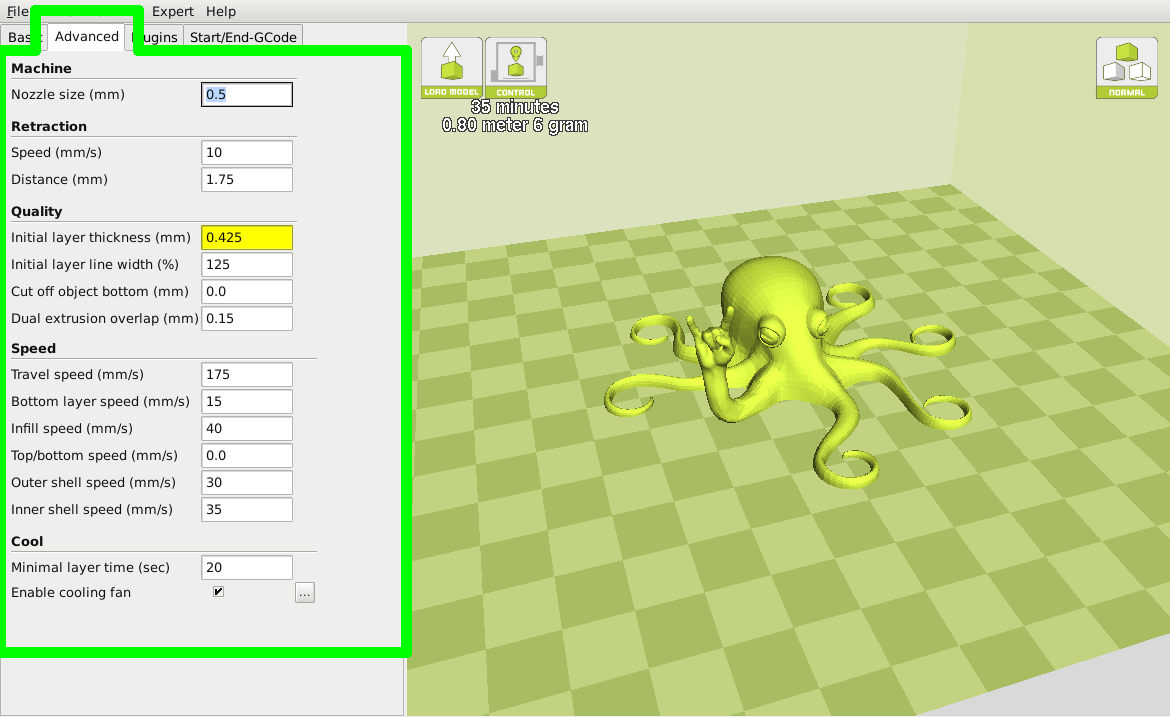
\includegraphics[keepaspectratio=true,angle=0,height=0.4\textheight,width=1.0\textwidth]{advancedtab.png}
\caption{View of Advanced Tab}
\label{fig:View of Advanced Tab}
\end{figure}

\subsection{\texttt{Nozzle Size (mm)}}
\index{Nozzle Size}
\index{Nozzle Diameter}
%%%% standalone version line %%%%
%This defines your nozzle size. The slicing engine uses this value combined with your other settings to determine how quickly to feed filament into your hot end, and how to generate the tool path. The TAZ ships with a 0.5mm nozzle standard. 

This defines your nozzle size. The slicing engine uses this value combined with your other settings to determine how quickly to feed filament into your hot end, and how to generate the tool path. \texttt{The Mini ships with a 0.5mm nozzle}.

\subsection{\texttt{Retraction Speed (mm/s)}}
\index{Retraction Speed}
Retraction Speed determines the speed at which your filament is reversed out of the hot end for travel moves and when changing direction during printing. We recommend keeping this set to less than 25mm/s to help protect the gears.

\subsection{\texttt{Retraction Distance}}
\index{Retraction Distance}
Retraction Distance determines how much filament is pulled out of your hot end on travel moves and when changing direction. You will want to adjust this depending on temperature settings and filament type. Higher thermal retaining filaments such as PLA behave better with a longer retraction distance. We have found anywhere from 1mm to 3mm is a good starting range.
% changed from "1 to 6mm" to remain conservative.

\subsection{\texttt{Initial Layer Thickness}}
\index{Initial Layer}
This will control how thick your first printed layer height is printed onto the heated bed. A larger initial layer height is more forgiving and will help first layer adhesion. All of our standard profiles have a 0.425mm initial layer height. This eliminates the need for adjustments when switching between filaments.  \textcolor{red}{Your LulzBot Mini automatic bed leveling system could be affected if you change this from the standard profiles. Adjust at your own risk.} If you want to change first layer "squish" see Z Offset \ref{ssec:Z Offset}, page \pageref{ssec:Z Offset} 

\subsection{\texttt{Initial Layer Line Width}}
\index{Initial Layer Width}
This will control how wide your first extruded filament path is for the initial layer. A wider line width will help with bed adhesion. We have found 125\% to be a good starting place. For models with moving, printed in place parts, a smaller initial layer line width is recommended. \textcolor{red}{Your LulzBot Mini automatic bed leveling system could be affected if you change this from the standard profiles. Adjust at your own risk.} If you want to change how much your first few layers "squish" to the sides, see Z Offset \ref{ssec:Z Offset}, on page \pageref{ssec:Z Offset} 


\subsection{\texttt{Cut Off Object Bottom (mm)}}
\index{Cut Off Object}
This setting is used to help print models that were not specifically designed for FFF printing. In particular, it is for models that do not have a flat surface to adhere to the plate. It will sink your object Xmm into the build plate, creating a nice flat surface to begin your print. You can also use this option to remove the lower portion of your model, or if carefully measured, cut your part in half for printing one object as two (or more) pieces. (Fig. \ref{fig:Cutoff Example}, page \pageref{fig:Cutoff Example})
\begin{figure}[H]
\centering
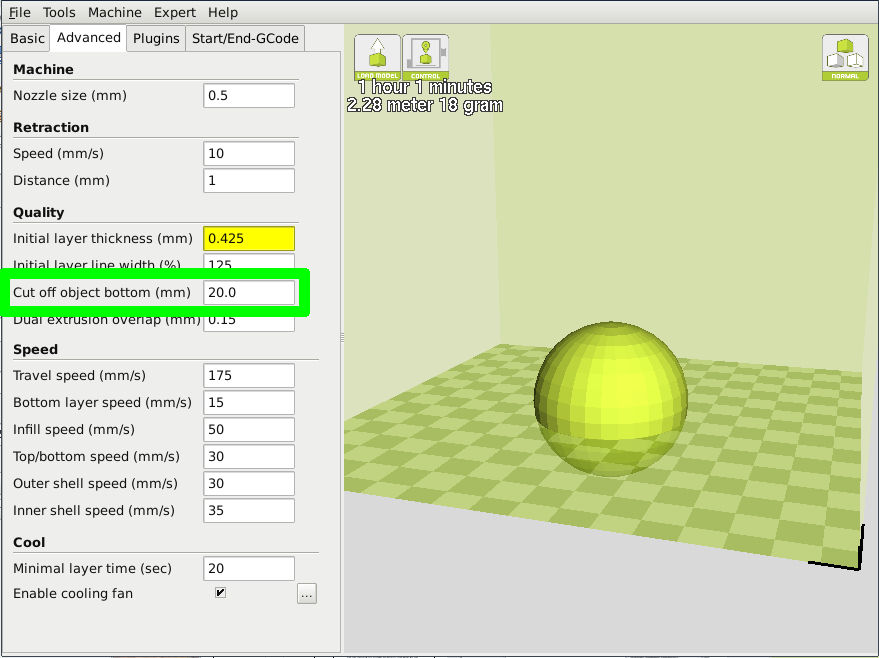
\includegraphics[keepaspectratio=true,angle=0,height=0.4\textheight,width=1.0\textwidth]{cutoff17.1.jpg}
\caption{Cutoff Example}
\label{fig:Cutoff Example}
\end{figure}

\subsection{\texttt{Dual Extrusion Overlap}}
\index{Dual Extrusion Overlap}
This will determine how far your Dual Extruders will overlap when laying down material. This will help adhesion between the two different colors or types of filament. This setting is only used when a printer is equipped with two hot ends and two extruders.

\subsection{\texttt{Travel Speed}}
\index{Travel Speed}
This setting will determine how fast your print head moves while not extruding filament. A normal travel speed of 125mm/s - 175mm/s is recommended.

\subsection{\texttt{Bottom Layer Speed}}
\index{Bottom Layer Speed}
This will control your initial layer speed. In general, a slower initial layer speed will help with first layer adhesion. 

\subsection{\texttt{Infill Speed}}
\index{Infill Speed}
This is how fast your print head speed will be while laying down the interior portion of your model. Faster speeds are usually tolerable here, as none of the infill will be visible from the outside of your object. If you go too fast compared to your inner and outer shells, you can have adhesion issues or globs of filament left behind from the print head.

\subsection{\texttt{Outer Shell Speed}}
\index{Outer Shell Speed}
This will be the outermost surface of the model. This is the most important speed setting, as it controls the speed of your print head on the visible layers. As a general rule of thumb, the slower you go the better looking print you will get. 

\subsection{\texttt{Inner Shell Speed}}
\index{Inner Shell Speed}
This affects vertical walls that are in between the outer shell and infill. This will not be visible but will help support the outer shell and the infill. We recommend keeping this speed setting between your infill speed and your outer shell speed.

\subsection{\texttt{Minimal Layer Time}}
\index{Minimal Layer Time}
This will determine a minimum amount of time your printer will spend laying down each layer. If your layer print time falls below this your printer will automatically slow down to reach this time before moving onto the next layer. Tweaking this can help get cleaner, crisper prints. If the tool head moves too slowly and lingers over the object, it can cause those areas to droop from excess heat, reducing final quality and finish. 

\subsection{\texttt{Enable Cooling Fan}}
\index{Enabling Cooling Fan}
Enables operation of your extruder active cooling fan. The fan settings can be adjusted in the \texttt{Expert Settings} options. See section \ref{sssec:Cooling} on page \pageref{sssec:Cooling} for details. In general, smaller parts will require more cooling for proper results. 

\section{\texttt{Plugins}}
\index{Cura Plugins}
Plugins are custom settings which will alter your print at specific points. The two that come preloaded with Cura are \texttt{Tweak at Z}, and \texttt{Pause at Height}. More plugins and information can be found here: \texttt{http://wiki.ultimaker.com/Category:CuraPlugin} To activate one of these highlight the desired plugin and click the drop-down arrow directly below the Plugins box. \textcolor{red}{These plugins affect how GCODE is generated. Use at your own risk.} \texttt{Be sure to turn these off before switching back to quick print mode. They will affect quickprint settings if left on.}

\begin{figure}[H]
\centering
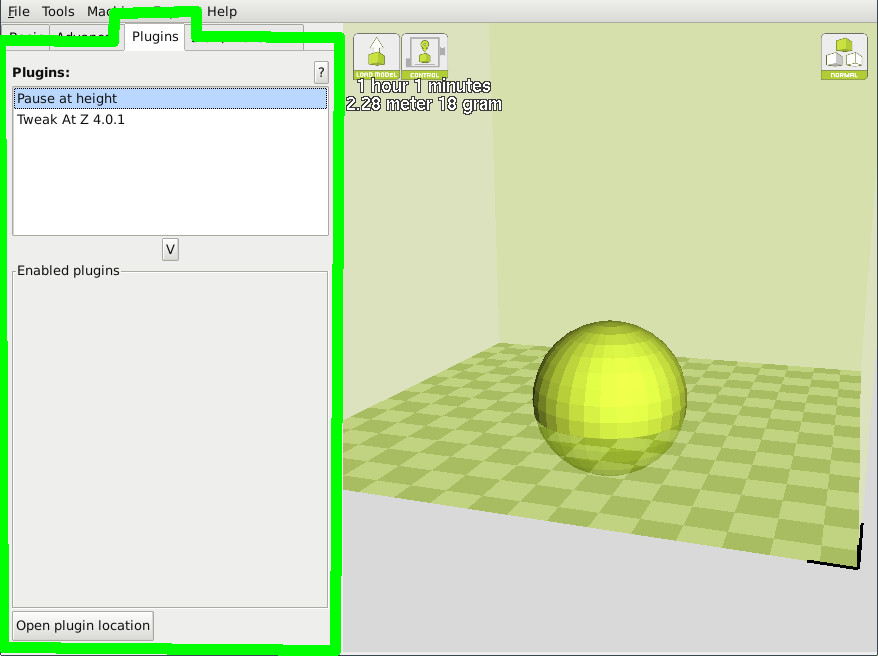
\includegraphics[keepaspectratio=true,angle=0,height=0.4\textheight,width=1.0\textwidth]{plugins17.1.jpg}
\caption{View of Plugins}
\label{fig:Plugins}
\end{figure}

\subsection{\texttt{Tweak at Z}}
\index{Tweak at Z Height}
Make basic changes at specified Z heights. You can define the Z height or layer count at which you want to make a change. Then choose how you would like to change your settings. You can alter temperatures, fan speeds, and print speeds. Fine tuning these for specific STL files, can produce cleaner prints.

\subsection{\texttt{Pause at Z Height}}
\index{Pause at Z Height}
Pause your print at a specified height. You can also specify where to move the print head and how much filament to retract. This will prevent “blobs” from accumulating on your print while paused. This setting is most commonly used when switching colors of filaments in the middle of a print.

\section{\texttt{Start and End Gcode Settings}}
\index{Custom Gcode}
\index{Start Gcode}
\index{End Gcode}
Custom Gcode allows for complex automatic printer movements and operations. By adding custom Gcode into the start or end of your file, you can alter how it prints. A comprehensive list of Gcode commands can be found here: \texttt{http://reprap.org/wiki/G-code} We recommend new users to leave this as provided in the profiles at \texttt{https://www.lulzbot.com/support/downloads}

%mini
\subsection{\texttt{Mini Specific Considerations}}
Please be cautious when changing any of these start and end GCODE settings. \textcolor{red}{This is where your automatic bed leveling commands are stored. If improperly altered, your printer will no longer automatically compensate for the heated bed position and can potentially damage components on the printer.} If you are uncertain of the change you are trying to make to start/end GCODE, please contact us at \texttt{Support@LulzBot.com} beforehand.

\definecolor{green2}{rgb}{0.00,0.375,0.0}

\subsection{\texttt{Changing Wiping and Probing Temperatures}} \label{sssec:num1}
\index{wiping temperature}
\index{probing temperature}
We have set wiping and probing temperatures that we have found work well with specific types of filament and filament manufacturers. \texttt{If you are using a type and/or manufacturer of filament not listed in the quickprint settings, you may need to adjust these temperatures for optimal probing.} In the start GCODE section, there will be three separate temperatures you can adjust. What these GCODE lines do will be described in the \textcolor{green2}{green text} to the right of the command. The ones you will want to adjust are:
\begin{itemize}
\item \texttt{M109 SXXX}                    \textcolor{green2}{; soften filament for z homing}
\item \texttt{M104 SYYY}                    \textcolor{green2}{; wipe temp}
\item \texttt{M109 SZZZ}                    \textcolor{green2}{; heat to probe temp}
\end{itemize}

By changing the variables \texttt{(XXX, YYY, ZZZ),} you can change what temperature your printer will soften, wipe, and probe. Our temperatures for softening, wiping, and probing will be a good starting point for other manufacturer's filament. When making adjustments, we recommend \texttt{+/- 5°C} changes at a time. \texttt{Be sure to watch the probing sequence when experimenting with new temperatures.}

\section{\texttt{Expert Settings}}
\index{Expert Settings}
\index{Full Settings}
Expert settings will give you more specific options for your retraction, skirt, active cooling, infill, support, brim, raft, and special settings. To gain access to this section you go to \texttt{Expert} > \texttt{Open Full Settings} or on your keyboard press \texttt{Control + E}.
\begin{figure}[H]
\centering
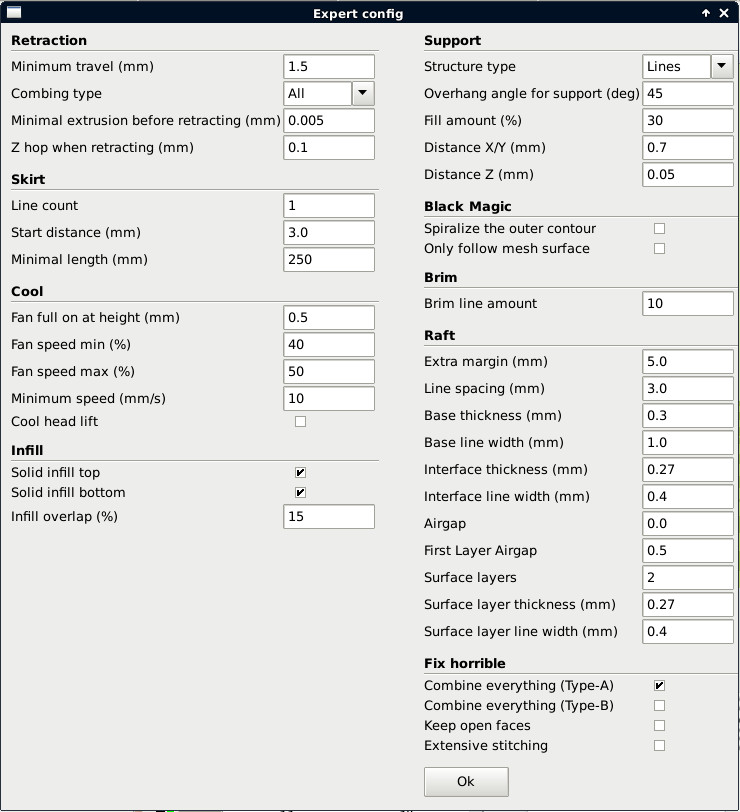
\includegraphics[keepaspectratio=true,angle=0,height=0.4\textheight,width=1.0\textwidth]{expert17.1.jpg}
\caption{View Expert Settings}
\label{fig:Expert Settings}
\end{figure}

\section{\texttt{Retraction}}
\index{Retraction}
\index{Stringing}
Retraction pulls filament out of your nozzle when it is not extruding to prevent your print head from dripping on your object. This section is where you will control how your extruder retracts its filament.

\subsection{\texttt{Minimum Travel}}
\index{Minimum Travel}
This sets the minimum travel distance of your print head in order to retract. If your print head is not moving at least this far during travel moves, it will not retract.

\subsection{\texttt{Combing}}
\index{Combing}
This option prevents your print head from traveling over holes in the X/Y plane when printing. This will slightly increase print time, but will prevent strings from getting caught on the holes during travel moves. We recommend keeping this setting on.

\subsection{\texttt{Minimal Extrusion Before Retracting}}
This will prevent a retraction move, if your extruder has input X mm of filament into the hot end. This is length of filament input into the hot end, not length extruded.

\subsection{\texttt{Z Hop When Retracting}}
\index{Z hop}
This will raise your print head Xmm while retracting. This setting helps prevent ooze and strings from being deposited on your print. 
%\textcolor{red}{We do not recommend this setting for TAZ 3 users and earlier. This can cause issues with Z dimensional accuracy.}

\section{\texttt{Skirt}}
\index{Skirt}
Skirt creates a line around the outside of your object. This is used to prime the extruder, in order to prevent missed filament at the beginning of a print. Leave this setting on. Turning this setting off will allow for utilizing the full build volume.

\subsection{\texttt{Line Count}}
\index{Line Count}
This will define the number of loops the Skirt creates around the outside of your object. Smaller models will require more loops to properly prime the extruder.

\subsection{\texttt{Start Distance}}
\index{Start Distance}
This will define the distance away from your model that the skirt will be created. The distance from the model will consume a portion of the maximum build volume in the X/Y plane.

\subsection{\texttt{Minimal Length}}
\index{Minmal Length}
This will define the minimum extruded line length for the skirt. This will override your line count, producing as many lines as required to reach the minimal length.

\section{\texttt{Cool}} \label{sssec:Cooling}
\index{Cooling}
\index{Fans}
This section will define how your extruder cooling fan will operate during the print. If your print speeds are slowed down due to minimal layer time, the fan will run between minimum and maximum speed based upon how much the layer is slowed down.

\subsection{\texttt{Fan on at Full Height}}
\index{Fan Settings}
This is your Z height where your fan will be turned on to its minimum percentage setting. Especially helpful with high temperature retaining filaments such as PLA. This will be scaled between 0\%, and your minimum fan speed based upon layer height; with it being disabled for the first layer.

\subsection{\texttt{Fan Speed Min}}
\index{Fan Settings}

This will be the speed your fan runs when enabled at full height. Once the Z height is reached for Fan on at Full Height, this will be the speed your fan runs at.

\subsection{\texttt{Fan Speed Max}}
\index{Fan Settings}
This is the fastest speed at which your fan will ever run. When your print speed is slowed down due to minimal layer time, your fan will run between minimum and maximum speed. The maximum fan speed is reached when your printer must be slowed by 50\% or greater.

\section{\texttt{Support}}
\index{Support Material}
You define how your support material is generated here. You must have some form of support turned on in the basic settings in order for these settings to have an effect.

\subsection{\texttt{Structure Type}}
\index{Support Settings}
You can choose between a Grid or a Line pattern for your support material. The grid will be a checkerboard pattern in the X and Y direction. The line option will produce lines in along the Y-axis for support. The grid will provide stronger support than the line option, but will be harder to remove.

\subsection{\texttt{Overhang Angle for Support}}
\index{Overhang Angle}
This will determine where support material is generated. In general you will be able to print a model with 45 to 90 degree angles in relation to the bed without support. A conservative setting for this is 45 degrees.

\subsection{\texttt{Fill Amount}}
\index{Fill Amount}
\index{support infill}
\index{support density}
This will determine how dense your support material is printed, similar to Infill Percentage. The higher the percentage, the better support, but it will be harder to remove the support material, will use more material, and will lead to a longer total printing time.

\subsection{\texttt{Distance X/Y}}
\index{Support X/Y}
This will determine how far away from your object in the X/Y plane that the support material is being placed. A larger distance entered here can make the material easier to remove, but it will not support as well.

\subsection{\texttt{Distance Z}}
\index{Support}
This will determine how far away your support material is from your object in the vertical direction. A smaller number here makes for better support, but makes it harder to remove.

\section{\texttt{Black Magic}}
\index{Black Magic}
This section allows you to transform your model into a hollow shell, a single layer thick.

\subsection{\texttt{Spiralize the Outer Contour}}
\index{Spiralize}
\index{Vase Mode}
This causes your Z-axis to be constantly moving upward as printing your single outer wall shell. The results are no layer change lines, giving a much smoother surface. This setting is typically only used for artistic objects as they will be fragile.

\subsection{\texttt{Only Follow Mesh Surface}}
\index{Follow Mesh Surface}
This will cause your print to follow the outside of your model, building it completely hollow with a single wall outer shell. This will also ignore the base layer, and the top layer. The difference between this and Spiralize, is that the Z-axis moves regularly. That is, it prints a layer and then moves up vertically to begin the next one.

\section{\texttt{Brim}}
\index{Brim}
Brim circles the base of the print while making contact, helping adhere the print to the heated plate. This is only one layer thick, and easily removed post-print. The distance around the base of the object will consume some of the maximum build volume in the X/Y plane. This section defines how the brim is formed when brim is activated in basic settings.

\subsection{\texttt{Brim Line Amount}}
This will determine the distance the brim will cover around the outside of your object. The more brim used, the better your part will adhere to the plate. 

\section{\texttt{Raft}}
\index{Raft}
Raft is a platform built underneath your object, designed to help adhesion and prevent warping. It will lay down support material, and then a platform on top of the supports. Your model will be built on top of this platform. The bottom surface of your printed part will not be as clean or as even when using this option. Raft is typically not required.

\subsection{\texttt{Extra Margin}}
\index{Extra Margin}
This determines the distance around the outside of your object that the raft is created. Can be helpful for ensuring no warping of the lower layers.

\subsection{\texttt{Line Spacing}}
\index{Line Spacing}
This will determine the spacing between “support” lines for the raft. A small spacing makes the support structures closer together improving strength of the raft, but uses more material.

\subsection{\texttt{Base Thickness}}
\index{Base Thickness}
This defines how thick your raft will be.

\subsection{\texttt{Base Line Width}}
\index{Base Line Width}
This will define how wide your “support” material is for the raft. This setting will determine how well the surface layers of the raft print.

\subsection{\texttt{Interface Thickness}}
\index{Interface Thickness}
This will determine how thick the surface layers of the raft are. The surface layers are the platform that is built upon the supports.

\subsection{\texttt{Interface Line Width}}
\index{Interface Line Width}
This will determine how wide the top layers of the platform will be. In general, you can keep this set to your nozzle size, as surface quality of the removable raft is not important.

\subsection{\texttt{Airgap}}
\index{Airgap}
This will define the distance between your raft and your print. A larger gap will make your part easier to remove, but will make the bottom of your print look worse.

\subsection{\texttt{Surface Layers}}
\index{Surface Layers}
This will determine the number of layers that create the “platform” of your raft. If you have a wide line spacing, you may want to increase this number to ensure a solid platform. 

\section{\texttt{Fix Horrible}}
\index{Fix Horrible}
These are some of the more advanced and experimental options. They are designed to help repair models with errors to make them suitable for 3D printing. \texttt{They do not always work.} Please be cautious when using these options as they can have unintended effects on your print quality.

\subsection{\texttt{Combine Everything (Type-A)}}
\index{Combine Type-A}
This will attempt to fix all external mesh errors, while keeping internal holes intact. This can accidentaly fill in intentional internal holes.

\subsection{\texttt{Combine Everything (Type-B)}}
\index{Combine Type-B}
This will ignore all internal holes of the model and only focus on the external holes. This is helpful when only the outside finish of the model is important.

\subsection{\texttt{Keep Open Faces}}
\index{Open Faces}
This will ignore all manifold errors in the object. It can create issues generating the GCODE as Cura does not know how to interpret the open holes. This option should only be used if you are sure that the holes in the mesh are intended. \texttt{In general, you should not use this option.}

\subsection{\texttt{Extensive Stitching}}
\index{extensive stitching}
This causes Cura to automatically add triangle meshes in an attempt to fix manifold errors. This algorithm will greatly increase GCODE generation time and may end up adding in un-intended meshes. It is recommended that you repair your model through MeshLab, FreeCAD or your preferred CAD program before attempting this option.

\begin{comment}
\section{\texttt{Dual Extrusion}}
\index{dual extrusion}
The LulzBot TAZ has the ability to add dual extrusion functionality with the Dual Extruder Tool Head. We only recommend the Dual Extruder Tool Head for advanced users. Installation and operation of the dual extruder will require you to flash your firmware, calibrate your extruders, level two heads to a single plane, define extruder offsets, and fine tune your slicing profile. This can be a little overwhelming for new users. We recommended that you have a couple of months of single extruder printing experience before making the switch. 

\subsection{\texttt{Tool Head Installation Instructions}}
\textcolor{red}{Refer to appropriate Dual Extruder Tool Head Quick Start Guide for the specific steps required to install and operate your new tool head. Failure to follow the proper steps may result in damage to the tool head or 3D printer.} Installation and operating instructions are available at \texttt{OHAI.LulzBot.com/accessories}. The following steps are only meant to be an overview of the typical process.

\subsection{\texttt{Updating Firmware}}
\index{updating firmware}
In order to use the Dual Extruder you will need to update your firmware to activate the second hot end.

\begin{itemize}
\item Power on your 3D printer and connect it to your computer through USB.
\item Select \texttt{Machine > Machine Settings}.
\item In the top right-hand corner you will see a \texttt{Change Tool Head} button, select this. 
\item Next you will need to select the proper hot end type. Please compare photos with your existing tool head. Choose the correct hot end and select \texttt{Next}.
\item Select the photo that corresponds with your tool head and press \texttt{Next}.
\item Select the appropriate tool head for your TAZ and select \texttt{Next}.
\item Choose the correct nozzle size for your machine. If you are not sure what size your printer has use your serial number to determine the nozzle size with the information found at \texttt{https://www.lulzbot.com/printer-identification}.
\item The final step will be \texttt{flashing the firmware}. Choose \texttt{Flash the firmware} to be sure to update the printers firmware to the proper settings. \textcolor{red}{This must be done to allow your printer to operate properly.}
\item Once the progress bar has completed select \texttt{OK > Next > Finish}.  
\item You can verify a proper firmware update by looking at the LCD screen. You should now see three separate temperature readings. 
\end{itemize} 
You can revert the firmware back to the stock configuration for your LulzBot 3D printer by selecting \texttt{Machine > Machine Settings > Change Tool Head}. Doing so will overwrite any of your current firmware settings.
\subsection{Preparing Cura}
In order to slice for a second tool head, you will need to let Cura know that you have added a second tool head. 
\begin{itemize} 
\item Select \texttt{Machine > Machine Settings > Extruder Count > 2}.
\item Select \texttt{Ok} to close out the screen.
\item Select \texttt{Machine > Machine Settings} to open the Machine settings again. 
\item A new section labeled \texttt{Extruder 2} is now present. Within it you will see an \texttt{X offset and Y offset}.
\item Set the \texttt{X offset to 0} and the \texttt{Y offset to -50}.
\item Select \texttt{Ok} to save your changes. The Machine settings window will close.
\end{itemize} 
\subsection{\texttt{Calibrating Extruders}}
\index{calibrating extruders}
Each individual extruder will have its own unique set of Extruder steps per unit, or Esteps. Your Dual Extruder was calibrated before leaving the production floor. The number for each extruder will be located on the back of the tool head. This will need to be updated within your printer's firmware.
\begin{itemize}
\item Load the outer and inner calibrations squares into Cura \texttt{https://www.lulzbot.com/downloads}
\item Open the Printer Interface window and set temperatures for both heads. Switch between hot ends by entering ``\texttt{T0}'' for the rear extruder into the command line terminal. Press \texttt{enter}.
\item Type ``\texttt{T1}'' for the front extruder into the command line terminal. Press \texttt{enter}.
\item Make two marks at 100mm and 120mm on the filament from the top surface of each extruder.
\item Once at the correct extrusion temperature type into the command line ``\texttt{G92}'' and press \texttt{enter}. Then ``\texttt{G1 E100 F60}'' and press \texttt{enter}.
\item Switch to the other tool head by entering ``\texttt{T0}'' for the rear or ``\texttt{T1}'' for the front. 
\item Type into the command line ``\texttt{G92}'' and press \texttt{enter}.
\item Type ``\texttt{G1 E100 F60}'' and press \texttt{enter}.
\item Measure the distance that the tool head over or under extruded. You will need to adjust your Esteps by 8 up or down for each mm it under or over extruded.
\item Update your Esteps for the rear extruder and E1steps for the front extruder through your LCD screen. \texttt{Configuration > Advanced Settings > E/E1 Steps > New Number}. Push in on the knob to exit out of the Esteps entry.
\item Store your new Esteps \texttt{Configuration > Store Memory}.
\end{itemize}

\subsection{\texttt{Level the Front Tool Head}}
\index{level dual extruder}
You will need to manually level the front hot end to the rear. This prevents the hot ends from hitting previously printed sections of your object during normal operation. 

\begin{itemize}
\item Home printer through the LCD screen. \texttt{Movement > Auto Home}
\item Move the Y axis back so \texttt{only} the rear hot end is over the bed plate. \texttt{Movement > Move Axis > 1mm > Y Axis}
\item Move the Tool Head down until the rear hot end is just touching the build plate. \texttt{Movement > Move Axis > 0.1mm > Z Axis}
\item Raise your front hot end by adjusting the M4 leveling screw on the front of the Tool Head.
\item Move your Y axis forward so the front hot end is over the plate. \texttt{Movement > Move Axis > 1mm > Y Axis}
\item Lower your front tool head using the M4 leveling screw. Your front head should just touch the bed plate as your rear hot end does.
\end{itemize}

\subsection{\texttt{Defining Second Extruder Offset}}
\index{second extruder offset}
To get crisper looking prints, you will want to really dial in your offsets. With the outer and inner square on your build platform, \texttt{left-click} on the outer square, then \texttt{right-click} on the inner square and select \texttt{Dual Extrusion Merge}. The red square will be printed with your front extruder, and the yellow square will be printed with the rear extruder.
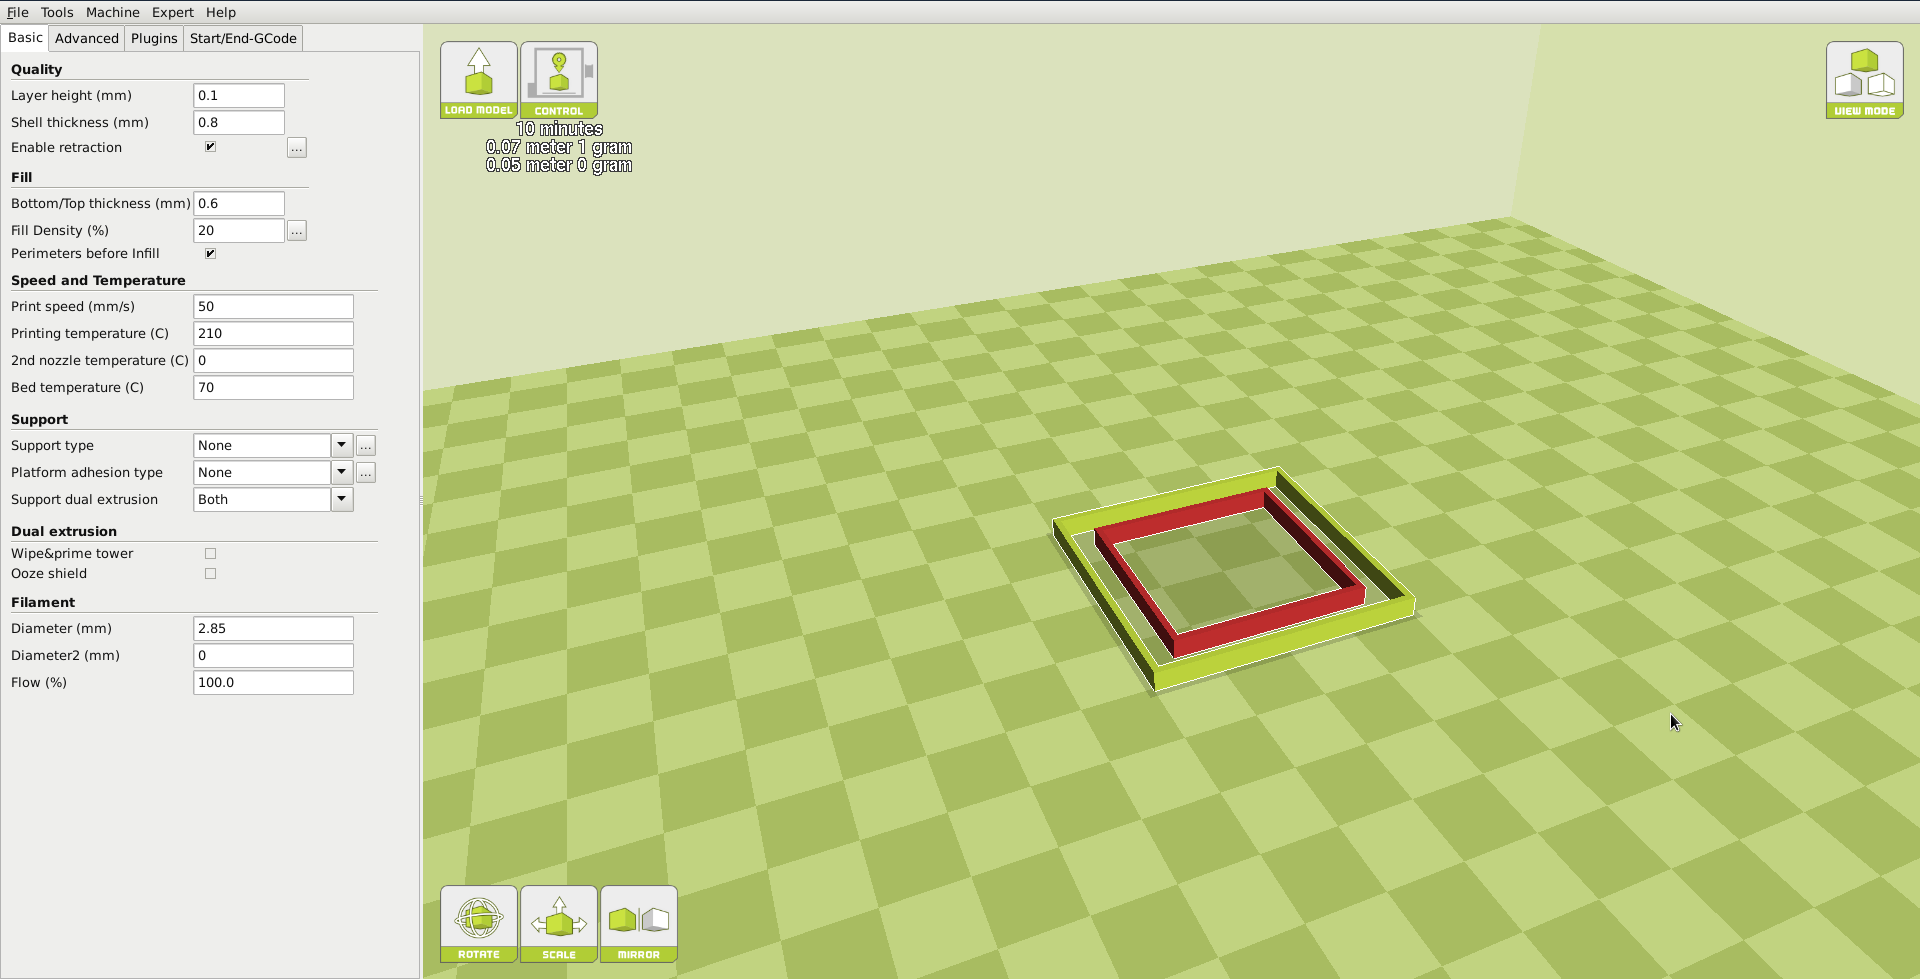
\includegraphics[keepaspectratio=true,angle=0,height=0.4\textheight,width=1.0\textwidth]{CalSquares1.png}
After printing the squares, you will want to measure Top, Bottom, Left, and Right gap. Enter these numbers into our offset calculator found here: \texttt{https://www.lulzbot.com/dual-extruder-calibration-calculator} This will produce new offsets, that will need to be updated in the Machine Settings menu. Repeat as many times as desired to truly fine tune the offset. 

\subsection{\texttt{First Dual Print}}
\index{first dual print}
When you are ready to produce your first dual extrusion print, you will need to combine the two separate STL files. One STL file will be for each print head. \texttt{Left Click} on whichever STL you would like printed with the \texttt{Rear Tool head}. Then \texttt{Right Click} on whichever STL file you would like printed with the \texttt{Front Tool head} and select dual extrusion merge. You will now see a single model in two colors on the build plate. The red section will be printed with the front extruder, while the green section will be printed with the rear extruder. 

\begin{figure}[H]
\centering
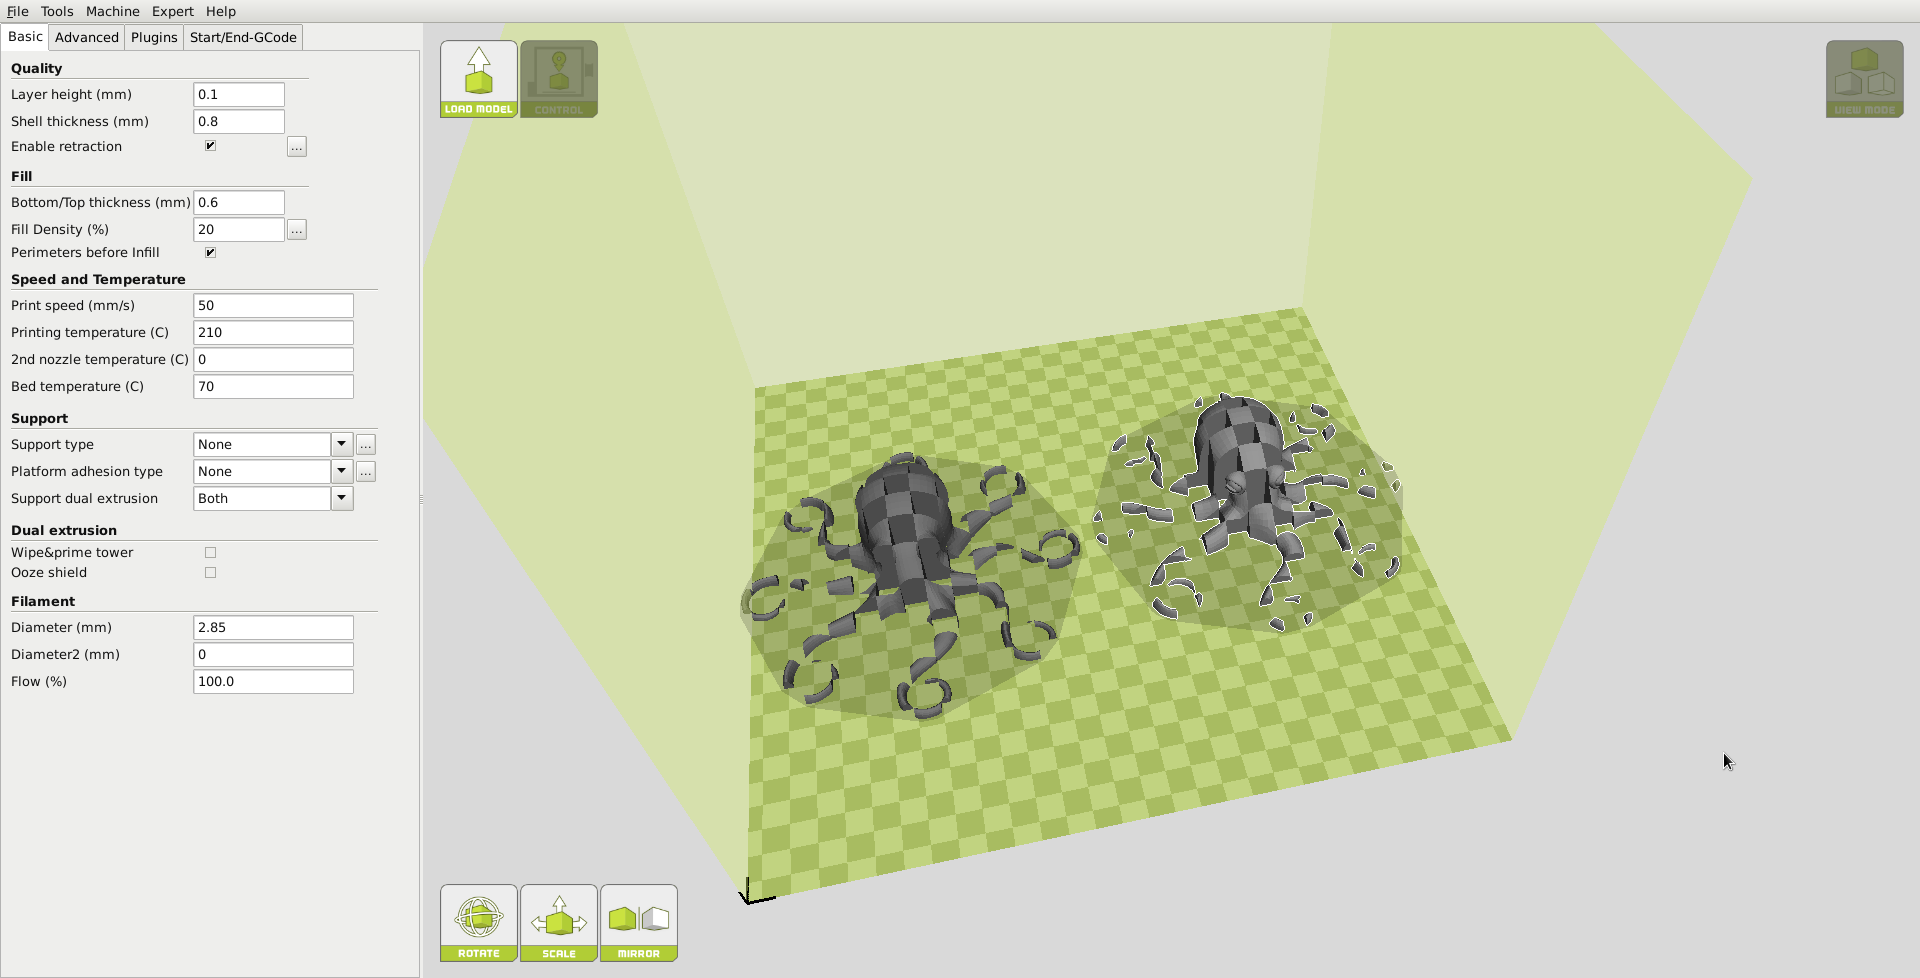
\includegraphics[keepaspectratio=true,angle=0,height=0.4\textheight,width=1.0\textwidth]{PreMerge.png}
\caption{Before Merge}
\label{fig:Before Merge}
\end{figure}

\begin{figure}[H]
\centering
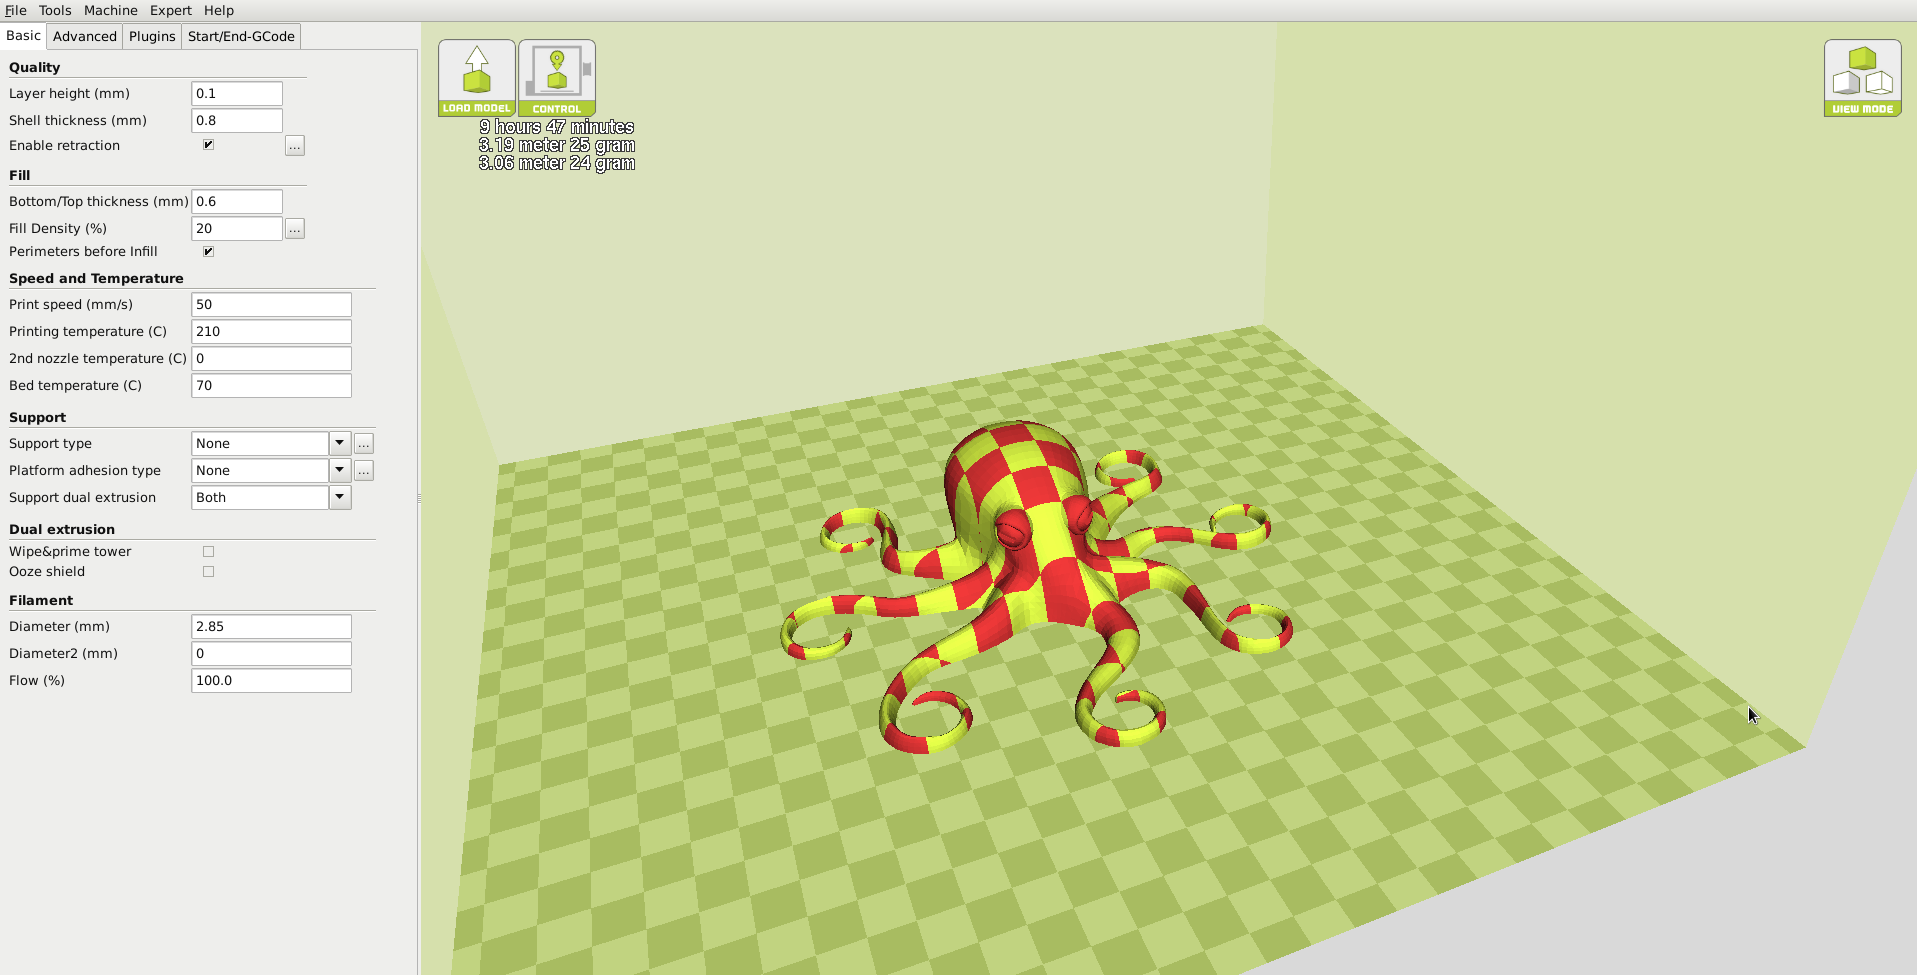
\includegraphics[keepaspectratio=true,angle=0,height=0.4\textheight,width=1.0\textwidth]{PostMerge.png}
\caption{After Merge}
\label{fig:After Merge}
\end{figure}

\subsection{\texttt{First Print}}
\index{First Dual Print}
After your object has been merged as intended, you will be ready to start the print. After selecting print from your SD card or the control panel, your printer will start the probing and cleaning process. It will clean both nozzles, but only probe with the rear. If you are getting contact with your printer nozzles on previous printed parts, you will need to check the level of the front hot end to the rear.

\end{comment}

